\documentclass[bachelor]{njupthesis}
\usepackage{tabularx}

\title{面向实体展览的沉浸式多模态交互系统设计与实现}
\author{沈立}
\advisor{刘思江}
\school{数字媒体与设计艺术学院}
\major{数字媒体技术}
\studentclass{B227103}
\studentid{B22710323}
\graduateyear{2026}
\begindate{2026年3月11日}
\finishdate{2026年6月14日}

\begin{document}

\makecover

\begin{chineseabstract}
随着虚拟现实、人工智能等数字技术的快速发展，人机交互正逐步从以键盘、鼠标为主的单一输入范式，转向融合多感知通道的沉浸式交互形态。然而，当前实体展览中的公共交互装置仍存在交互方式趋同、情感反馈缺失、体验深度不足等问题。本文针对上述问题，设计并实现了一套面向实体展览的沉浸式多模态交互系统。系统以Unity引擎为核心交互平台，整合了手势识别、面部情绪识别、交互应用状态感知等多源信息，并基于大语言模型智能体（Qwen3.6 + DeepAgent）构建中央决策模块，实现对虚拟场景与物理装置（LED灯阵、音效等）的协同控制。本文详细阐述了系统的总体架构、网络通信协议、智能体工具调用机制、关键视觉与交互模块的实现方法，并展示了实体装置的设计与集成。本系统为构建更具情感连接与沉浸感的公共展览交互体验提供了可行的技术路径与设计参考。

\chinesekeyword{多模态交互；游戏引擎；智能体；情感计算；实体展览}
\end{chineseabstract}

\begin{englishabstract}
With the rapid development of digital technologies such as virtual reality and artificial intelligence, human-computer interaction is gradually shifting from a single input paradigm dominated by keyboards and mice to an immersive interaction paradigm that integrates multiple sensory channels. However, current public interactive installations in physical exhibitions still suffer from homogenized interaction methods, lack of emotional feedback, and insufficient experience depth. To address these issues, this thesis designs and implements an immersive multimodal interaction system for physical exhibitions. The system uses Unity engine as the core interaction platform, integrating multi-source information such as gesture recognition, facial emotion recognition, and application state perception, and constructs a central decision-making module based on large language model agents (Qwen3.6 + DeepAgent) to achieve coordinated control of virtual scenes and physical devices (LED arrays, sound effects, etc.). This thesis elaborates on the system's overall architecture, network communication protocols, agent tool-calling mechanisms, implementation methods of key visual and interaction modules, and demonstrates the design and integration of physical devices. This system provides a feasible technical path and design reference for constructing more emotionally connected and immersive public exhibition interactive experiences.

\englishkeyword{Multimodal Interaction; Game Engine; Agent; Affective Computing; Physical Exhibition}
\end{englishabstract}

\thesistableofcontents

\thesischapterexordium

\chapter{绪论}

\section{研究背景}

在日常的数字交互中，无论是个人电脑上的电子游戏，还是移动设备上的各类应用，人们的交互方式长期依赖键盘、鼠标、手柄或触摸屏等传统输入设备，而系统的反馈也大多局限于屏幕内部的视觉变化与扬声器发出的音效；而另一方面，当谈及沉浸式体验时，公众的第一反应又往往将其与虚拟现实头戴设备联系在一起，似乎只有将用户从物理空间中完全剥离、置入一个由头显构建的虚拟环境，才称得上真正的沉浸。然而，这种将沉浸式体验与虚拟现实等同的认知恰恰忽略了实体空间本身所具有的不可替代价值。在博物展览与公共艺术装置等真实场景中，参观者身处物理空间，其身体在场性、空间感知能力与多感官协同体验是任何头戴式设备无法完全复现的。更重要的是，实体展览中的参观者无需佩戴额外设备即可自然移动、观察和感受，其社交行为不受遮挡，使得多人共享体验以及更深刻的情感联结成为可能。

从当今实体展览的发展态势看，其也正亟待引入更具沉浸的交互方式。公共交互装置作为现代城市空间与博物展览中的新兴艺术表达媒介，致力于构建人与作品之间的深度对话\citing{wen2022huadong}。当今的展览模式正逐渐从藏品陈列和静态信息呈现，向强调观众参与和体验感受的方向演进，博物馆等机构也持续致力于打破“请勿触摸”的传统禁锢，转而追求更具实践性、叙事性与沉浸感的互动体验\citing{ogrizek2024vr}\citing{jiang2024dunhuang}\citing{pietroni2025multisensory}。但遗憾的是，当前展览中的公共交互装置在交互体验上仍存在明显不足：一方面，部分系统仅简单引入数字屏幕与触控交互，参观者的体验与操作普通电子设备无异，未能充分发挥实体展览特有的现场感与空间优势；另一方面，由于设计范式趋同，许多装置的交互方式、反馈逻辑与视觉表现呈现同质化倾向，难以有效促进参与者的情感提升\citing{wen2022huadong}与持续探索，导致可互动但不耐体验的现象。这使得互动装置未能充分实现其作为展览媒介应有的情感沟通与意义建构价值，观众与作品之间难以建立稳定而深入的联系。

事实上，在此前已有少数先锋艺术家与商业团体尝试将沉浸式体验带入真实物理空间，但这些探索大多发生在人工智能技术爆发式跃迁的前夜，其交互逻辑仍受限于预设规则与固定脚本。而近两年来，随着大语言模型与视觉语言模型的飞速发展，尤其是2026年初，以OpenClaw为代表的个人终端智能体火爆互联网的当下，这种根植于现实空间的沉浸式体验也被赋予了全新的可能。


\section{研究目的和意义}

本课题旨在借助人工智能与智能体技术，将游戏引擎与其所支撑的高品质沉浸式交互体验带到实体展览空间之中，为此设计并实现了沉浸式多模态交互系统及其配套交互应用《回声之境》。具体而言，本课题探索了一种将手势与面部表情纳入输入模态、将多模态智能体作为核心多模态理解模块、将现实三维空间中的LED灯阵变化与屏幕空间内的动态视觉生成协同作为输出反馈的新型交互范式。参展者的手势动作与情绪状态被实时感知，驱动虚拟场景内的角色移动和视觉动效生成，同时通过物理灯光装置将这种变化延伸至实体展览空间，使沉浸感从屏幕内部扩散至物理世界。

人类的情感状态与行为意图天然地外化于面部表情、手势与身体姿态之中。深度学习在计算机视觉与运动捕捉领域的持续突破，使得对这些具身化信号的实时捕获与高精度解析已经非常成熟。借助Google推出的MediaPipe解决方案，可在Android、iOS、网页和Python应用中快速应用手势识别、面部特征点检测等任务\citing{google2024mediapipe}。与此同时，大语言模型与视觉语言模型的快速演进，赋予了多模态智能体跨模态理解、任务规划与工具调用的综合能力\citing{durante2024agent}。这种能力恰好填补了感知与执行之间的认知鸿沟：智能体接收视觉系统捕获的手势与表情信息，结合上下文进行意图推理与情感判断，进而生成对虚拟场景与物理设备的协同控制指令，形成“感知—理解—反馈”\citing{yao2023react}的闭环。传统多模态情感识别研究已表明，融合面部表情与身体姿态等多通道信号能够显著提升情感理解的准确性与鲁棒性\citing{tao2024multimodal}，而本课题将这种理解进一步延伸为对环境的具身化改造——手势与表情由此超越传统的控制指令语义，成为人机之间一种更自然、更具情感深度的沟通语言。

在交互应用的开发平台的选择上，Unity引擎凭借其成熟的实时渲染管线、场景管理系统与物理模拟能力，能够在消费级硬件上维持交互帧率下的高品质视觉输出。更为关键的是，游戏产业在数十年的发展历程中积累了丰富的空间交互、叙事引导与即时反馈的设计经验，这些经验可以直接反哺展览系统的交互设计\citing{kruger2024gameengines}。将游戏引擎引入实体展览场景，本质上是将虚拟世界中打磨成熟的交互循环移植到物理空间之中，使展览体验获得游戏般的趣味性与沉浸深度。

这种以多模态智能体为认知核心、以手势与表情为输入通道、以物理灯光与虚拟画面为双重输出的交互范式，回应了当前展览交互装置面临的核心困境。本课题通过智能体的统一调度，将参观者的情感信号、虚拟场景的视觉生成与物理灯阵的空间渲染纳入同一控制闭环，使三者协同变化、彼此呼应，构建出一种屏幕内外相互渗透、虚实交融的沉浸式体验。围绕实体展览场景开展上述设计研究，对于重构用户体验范式、创新情感反馈机制、探索人工智能与游戏引擎在非游戏场景中的融合应用具有重要的现实意义。

\section{国内外研究现状}

\subsection{实体展览中的交互装置实践}

在实体展览交互装置领域，国际性跨域艺术团队teamLab以其基于自研引擎的实时视觉演算而著称。如图\ref{fig:teamlab-exhibition}所示，teamLab在沉浸式展览中基于自研引擎实时演算生成花朵的绽放、瀑布的流淌、蝴蝶的路径等视觉效果，并且会根据观众互动实时改变\citing{teamlababout}。他们在世界各地举办了艺术展并开设了多处大型常设美术馆，其展览作品被世界各大艺术机构收藏，代表了沉浸式展览的技术前沿。

\begin{figure}[htbp]
  \centering
  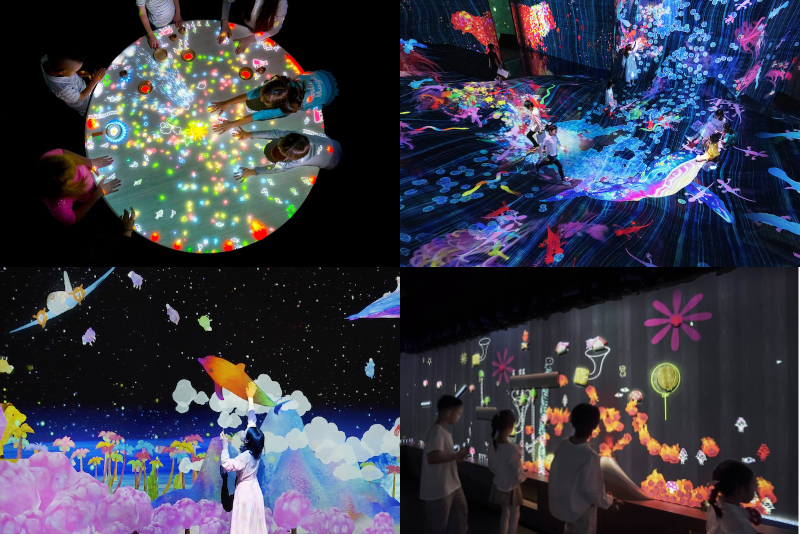
\includegraphics[width=0.8\textwidth]{pic/teamLab.jpg}
  \caption{teamLab团队的沉浸式展览交互作品}
  \label{fig:teamlab-exhibition}
\end{figure}

国内方面，博物馆等文化机构也在积极探索虚实联动的交互装置应用。如图\ref{fig:liangzhu-interactive}所示，位于浙江省杭州市余杭区的良渚博物馆内已部署虚实联动的交互装置，允许参观者通过操作实体装置与虚拟场景互动\citing{ogrizek2024vr}，体现了实体展览中虚实联动的交互理念。这一案例表明，将实体操作与虚拟反馈相结合的交互模式在国内博物馆场景中已得到初步应用。然而，此类装置大多仍停留在“触发—响应”的简单交互层面，即参观者执行特定操作后触发预设的视觉或听觉反馈，系统尚不能根据参观者的情绪状态、交互历史或行为特征进行动态的、个性化的响应调整。

\begin{figure}[htbp]
  \centering
  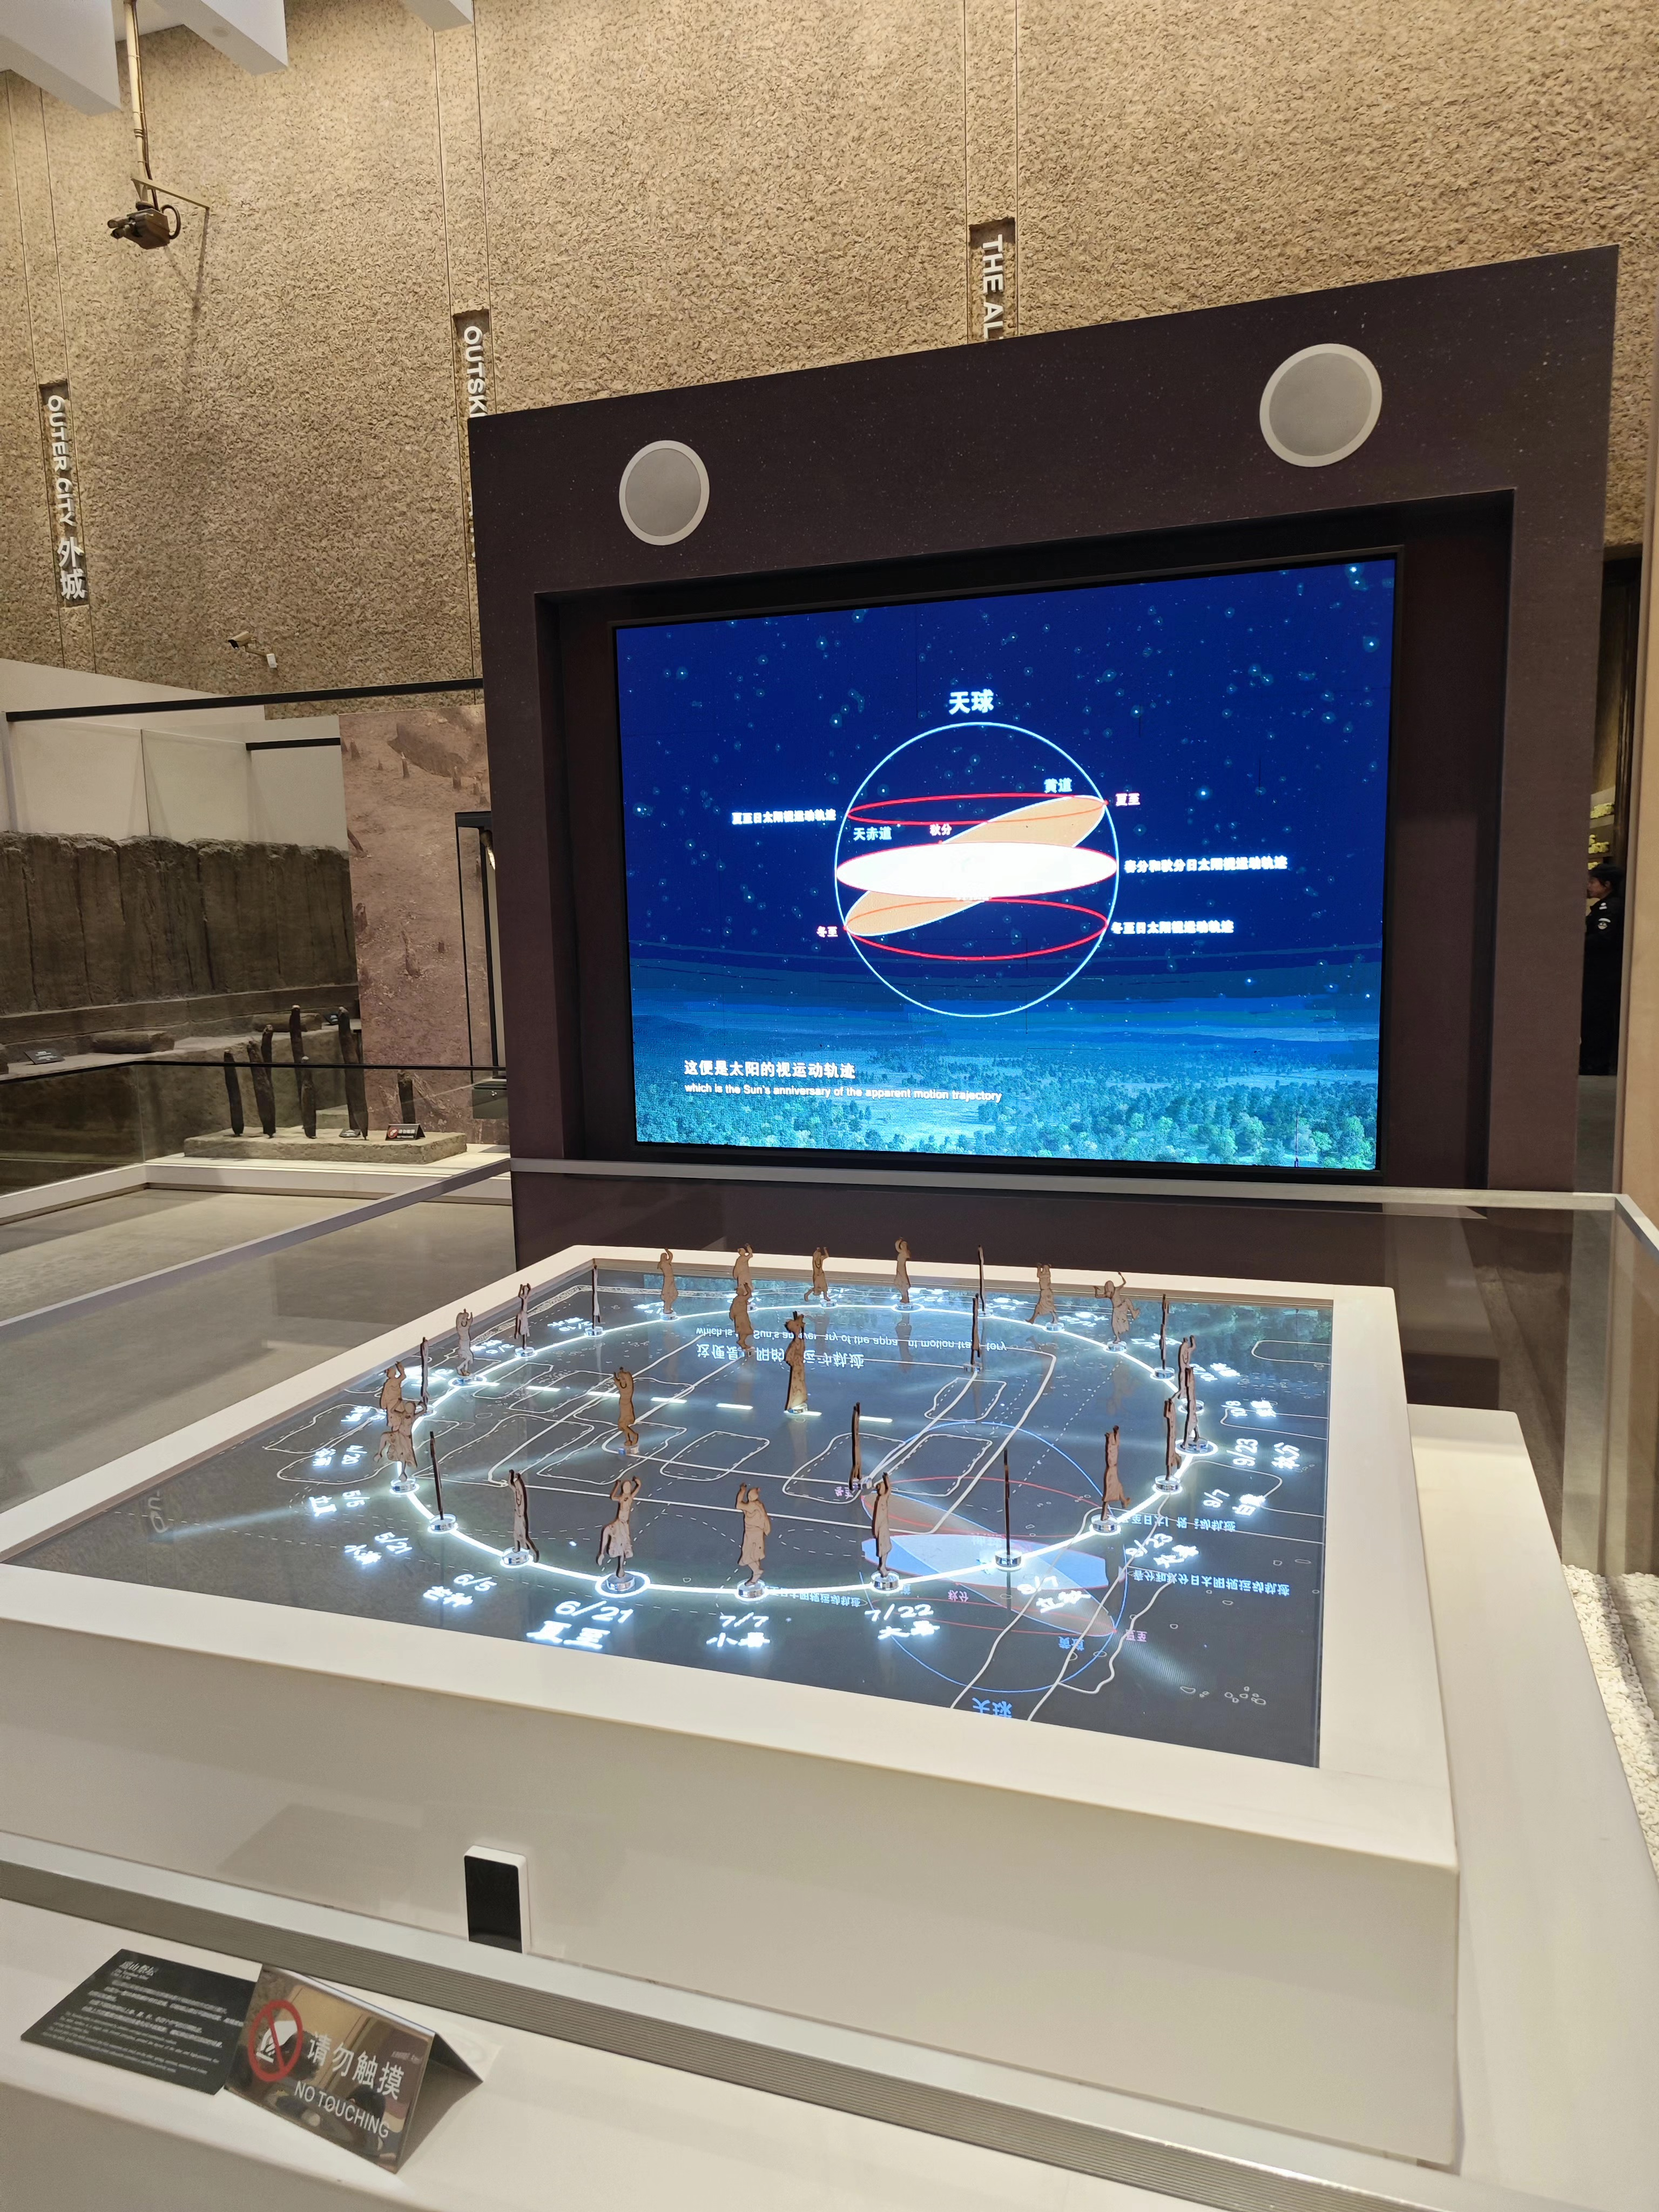
\includegraphics[width=0.5\textwidth]{pic/IMG_20260405_120402.jpeg}
  \caption{良渚博物馆内的交互装置}
  \label{fig:liangzhu-interactive}
\end{figure}

\subsection{虚拟沉浸式体验的前沿探索}

在虚拟沉浸式体验领域，游戏引擎技术与人工智能的融合正在催生全新的交互范式。Epic Games公司在《堡垒之夜》中举办的虚拟演唱会是一个标志性案例。如图\ref{fig:epic-concert}所示，该演出通过根据音乐内容实时改变场景Shader与后期处理参数，实现了富有感染力的视听体验，取得了良好口碑和极为可观的传播效果\citing{epic2024niagara}。这一案例展示了游戏引擎在实时视觉生成方面的强大能力，以及程序化内容生成在大型虚拟演出中的应用潜力。然而，虚拟演唱会本质上仍是一种单向的视听呈现——观众是信息的被动接收者，系统并不感知个体观众的状态，也无法根据观众反应进行实时调整。

\begin{figure}[htbp]
  \centering
  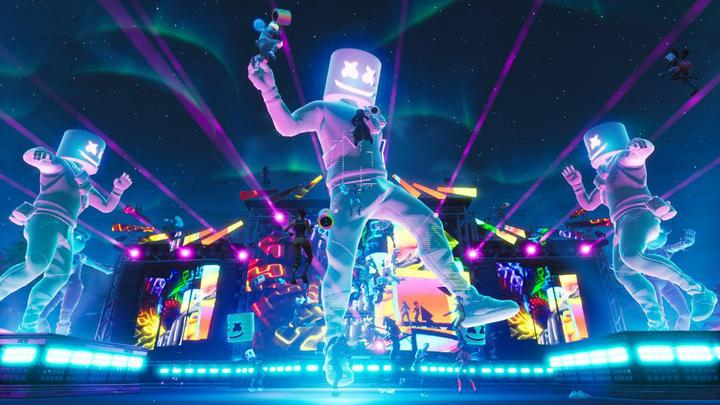
\includegraphics[width=0.8\textwidth]{pic/堡垒之夜.jpg}
  \caption{《堡垒之夜》虚拟演唱会}
  \label{fig:epic-concert}
\end{figure}

在多模态AI驱动的交互叙事方面，Anuttacon公司于2025年推出的《Whispers from the Star》\citing{whispersfromstar}代表了当前的技术前沿。如图\ref{fig:whispers-from-star}所示，该作品采用先进的多模态AI技术，玩家以语音形式与被困外星球的角色Stella实时互动。借助100\%实时渲染技术，Stella的对话、表情与动作均由AI根据对话内容动态生成，且玩家的选择会直接影响故事走向，而非遵循预设的对话分支。这种全新的叙事交互范式为玩家带来了前所未有的沉浸感，也开创了AI驱动交互叙事的新方向。

\begin{figure}[htbp]
  \centering
  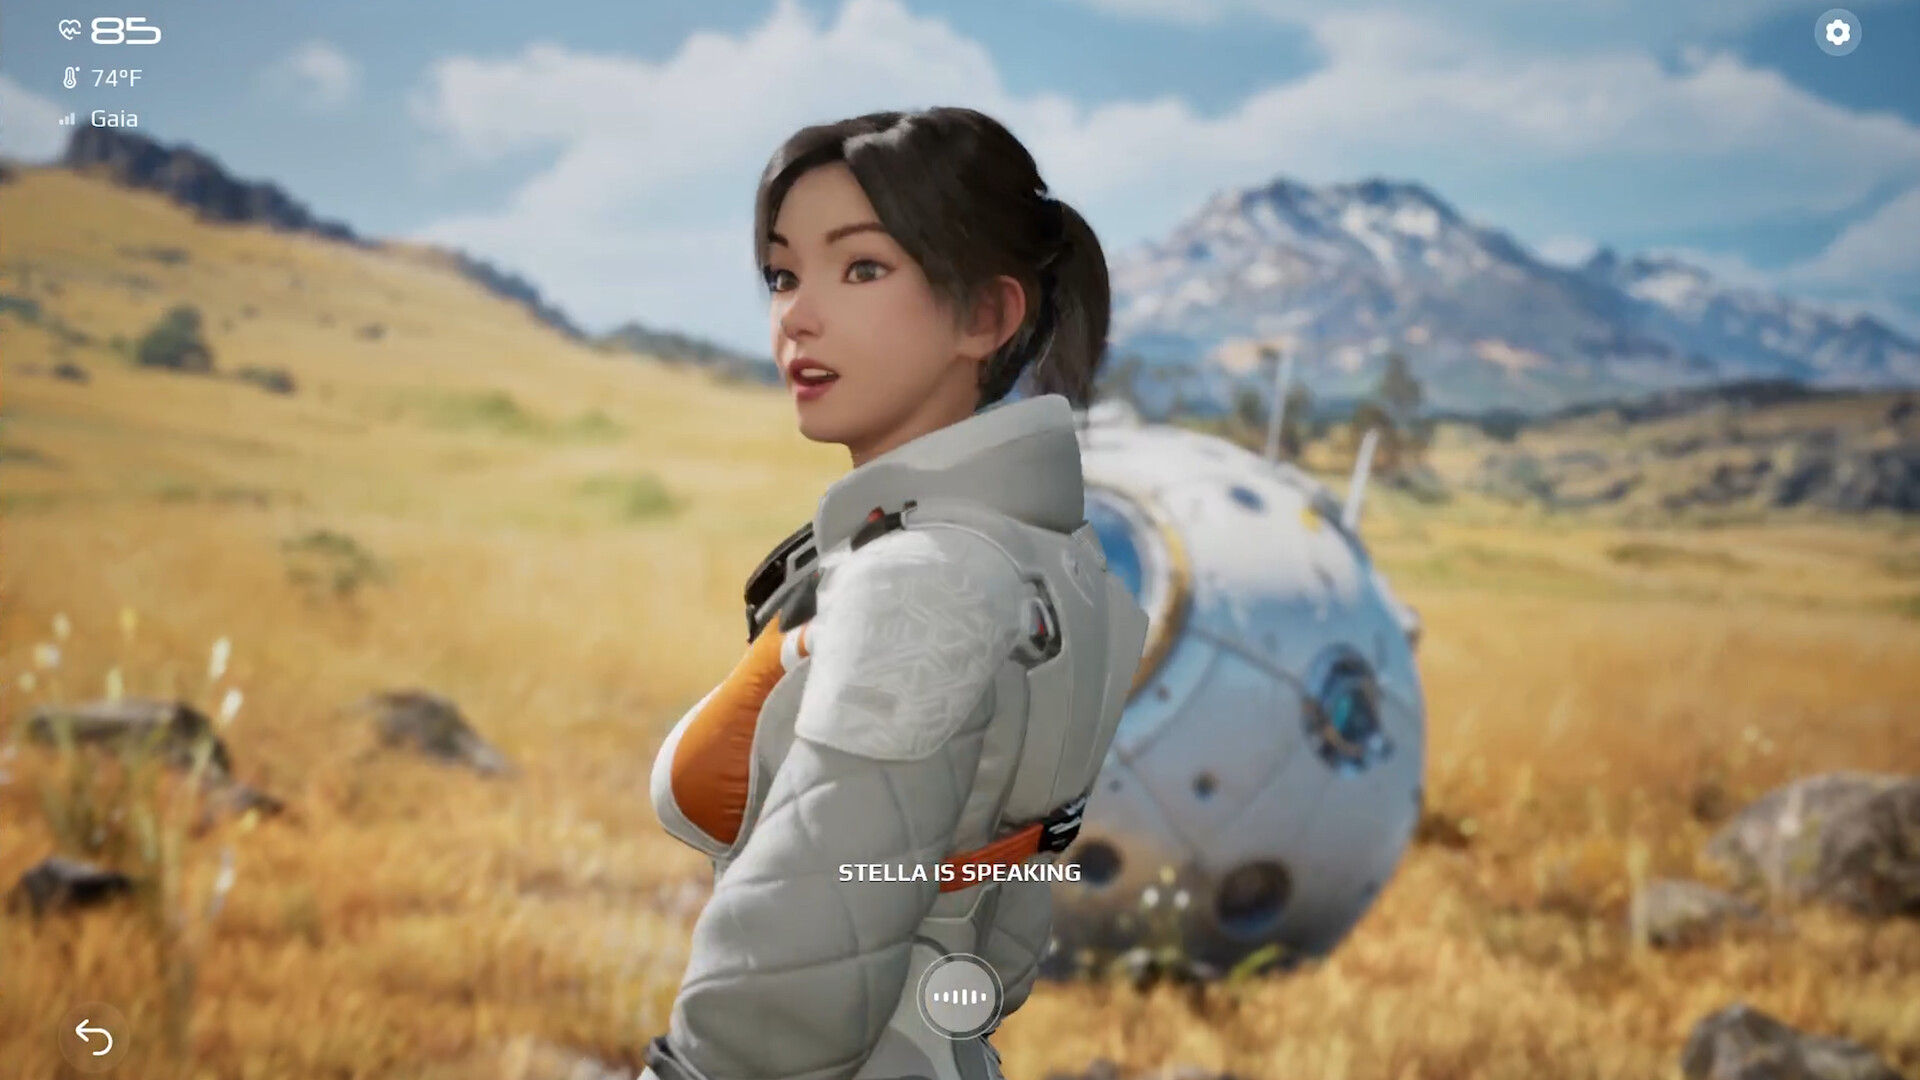
\includegraphics[width=0.7\textwidth]{pic/Whispers from the Star 1920x1080.jpg}
  \caption{《Whispers from the Star》游戏界面}
  \label{fig:whispers-from-star}
\end{figure}

\begin{figure}[htbp]
  \centering
  \includegraphics[width=0.8\textwidth]{pic/LPM1.0.png}
  \caption{LPM 1.0（Large Performance Model）}
  \label{fig:lpm}
\end{figure}

2026年，研究团队发布的LPM 1.0（Large Performance Model）\citing{lpm2026}将视频角色表演与全双工对话深度融合，能够以文本、音频和图像为多模态控制信号，实时生成在倾听、说话与静默三种状态下均保持身份一致性的角色视频，为对话式智能体提供了视觉表演引擎。这一技术突破使得AI角色能够在完整的交互状态循环中保持一致的身份表现，显著提升了虚拟角色的真实感与可信度。

\subsection{现有实践的启示与本课题的切入点}

综合来看，上述国内外实践在各自领域均已达到令人瞩目的高度：teamLab证明了物理空间中实时视觉演算的艺术感染力，《堡垒之夜》虚拟演唱会展现了游戏引擎在大型实时呈现中的技术成熟度，《Whispers from the Star》与LPM 1.0则揭示了AI驱动交互叙事的全新可能。

这些工作无一不让人印象深刻，但它们的交汇地带仍是一片尚待探索的空白。如果将物理展览空间的现场感、游戏引擎的实时交互能力与多模态智能体的情境理解能力置于同一系统之中，又会产生怎样的交互体验？实体展览中的参观者能否通过手势与表情与虚拟场景进行更自然、更具情感深度的沟通？虚实双重输出通道在实际交互中会产生怎样的协同效应？这些问题正是本课题试图回答的核心。

\section{论文内容安排}

本论文后续的内容安排如下：

第二章为文献综述，从实体展览交互装置、游戏引擎沉浸式体验技术及多模态交互与智能体技术三个方面进行详细的技术调研与评述；

第三章为需求分析与总体设计，明确系统核心需求，阐述交互设计理念与艺术设计，并给出总体架构与通信协议设计；

第四章详细描述关键技术与各模块的实现方法，包括智能体EchoAgent、TCP通信与并发控制、虚拟场景与视觉呈现以及虚实联动控制；

第五章为应用场景演示与测试，展示系统在实际展览中的部署效果并进行功能、性能测试与交互体验评估；

第六章总结全文工作，归纳主要贡献与创新点，并反思不足。

文末附有结束语、致谢、参考文献及附录。

\chapter{文献综述}

本课题旨在构建一套面向实体展览的沉浸式多模态交互系统，以多模态智能体为认知核心、以游戏引擎为交互平台、以物理灯光装置为虚实联动载体。围绕这一目标，本章从实体展览交互装置、游戏引擎沉浸式体验技术与多模态交互智能体三个方向展开文献调研——三者分别对应了系统的交互设计基础、视觉呈现平台与智能决策核心。

\section{实体展览交互装置研究进展}

一套完整的博物馆交互展览系统通常包含数据层、逻辑层与展示层三层架构。展示层负责提供高保真的三维渲染与多模态交互界面，是参观者与展览内容发生直接接触的界面层，也是本课题聚焦构建与优化的核心层级\citing{li2024exhibition}。

互动装置艺术作为连接展览内容与观众的关键媒介，其核心价值在于重塑观演关系。在传统剧场中，表演者与观众同时在场的等级制度清晰可辨；而在数字表演中，创作者往往是隐身的，观演者从被动的“观看者“转变为能够成就甚至重塑表演的“参与者”\citing{lu2024digital}。英国导演戴维·布莱尔1993年的线上电影《蜡网》（WAXWEB）提供了早期范例：这部85分钟的作品被拆分为8万个零散单元，观众可以在任意时刻通过“超视频“按键自行拼凑碎片、构建叙事，从而获得观影主动权——媒介不再只是信息的载体，而是赋予了观演者共创的可能\citing{lu2024digital}。

随着虚拟现实与人工智能技术的介入，数字表演中的互动性被进一步深化。VR将观者的参与性从架上的“画外“升华至虚拟现实的“画内”，沉浸式体验不再仅是一种视觉奇观，更是一种身体在场的感知方式。蒋旎等人围绕敦煌艺术展开的沉浸式展览实践为这一方向提供了具体参照\citing{jiang2024dunhuang}：在“遇见当代飞天“主体展演空间中，随着参观者位置移动，投影区域相应位置实时生成雷达交互后的粒子渲染画面，形成视频画面层与动态实时渲染层叠加的沉浸效果。这一实践表明，数字人文研究成果正从文本数据转化为具有场域感、以全息与沉浸式为体验特点的艺术语言。

在国际层面，Pietroni等学者围绕博物馆多感官交互体验开展了系统研究：其主导的IntARSI项目探索了基于自然用户界面的博物馆交互设计方法，整合手势、触觉与听觉等多通道感知\citing{pietroni2021accessibility}；在此基础上，其近期研究进一步提出了面向混合现实与多感官叙事的博物馆体验框架，主张物理空间与数字内容的深度融合是下一代博物馆体验的核心方向\citing{pietroni2025multisensory}。

互动仪式链理论从设计层面为上述实践提供了系统的组织框架\citing{wen2022huadong}。温文龙等学者指出，通过预设具有规范性、表演性与趣味性的互动仪式，可以为参与者创造特定的体验情境——在仪式化的互动过程中，情感能量得以产生、分享与传递，并通过“仪式链”的连续性维持高强度的参与体验。如图\ref{fig:ritual}所示，这一理论将展览体验解构为一系列可设计的情感阶段，每个阶段的交互机制与视觉反馈均服务于相应的情感目标。

\begin{figure}[htbp]
  \centering
  \includegraphics[width=0.8\textwidth]{pic/互动仪式理论与互动装置的要素适配.png}
  \caption{互动仪式理论与互动装置的要素适配\citing{wen2022huadong}}
  \label{fig:ritual}
\end{figure}

在具体的设计语言层面，情感化设计将人的情感需求置于设计的首位\citing{norman2005emotional}。李静雅等人通过TouchDesigner软件实验，提出了节奏与视觉形态关联的音乐可视化模型——圆形对应慢节奏、方形对应中节奏、三角形对应快节奏\citing{li2023music}，为视听联觉反馈提供了可操作的映射规则。Valérian Fraisse等人则从艺术意图、交互设计与系统设计三个视角出发，提出了描述交互式声音装置的概念框架\citing{fraisse2021sound}。实体工具在沉浸式交互中的作用同样值得关注：研究表明，在博物馆VR交互中为复杂任务提供实体操作工具能对用户体验产生积极影响\citing{ogrizek2024vr}。

总体而言，数字表演与沉浸式展览的发展历程清晰地勾勒出一条互动性不断深化的轨迹：从互联网艺术赋予观众的叙事选择权，到VR技术实现的“身体在场”，再到AI驱动下由观众行为实时生成的视觉响应——每一次技术跃迁都在拉近观者与作品之间的距离。这一演进方向直接定义了本课题的设计目标：构建一个能够感知参展者行为与情绪、并据此实时生成个性化视觉与物理反馈的交互系统。


\section{游戏引擎在沉浸式体验中的技术应用}

视觉生成作为一种交互实践，其探索可追溯至20世纪70年代。J. B. Mitroo等人采用彩色光栅图形显示器，将音符、和弦及和弦进行转化为可视化图像，如图\ref{fig:1979music}所示\citing{mitroo1979music}。尽管受限于当时的硬件条件，这项早期工作已经触及了音乐与视觉之间映射关系的核心命题——什么样的声音对应什么样的视觉形态——这一问题至今仍是交互艺术设计中的基础课题。

\begin{figure}[htbp]
  \centering
  \includegraphics[width=0.6\textwidth]{pic/1979music.png}
  \caption{J. B. Mitroo 等人的音乐可视化图像}
  \label{fig:1979music}
\end{figure}

经过数十年的技术演进，游戏引擎已发展为构建沉浸式虚拟环境的核心工具。Unity与Unreal Engine等引擎集成了图形渲染、物理模拟、音频处理与脚本逻辑等功能模块，极大降低了复杂交互应用的开发门槛\citing{kruger2024gameengines}。在本课题所关注的展览交互场景中，游戏引擎的价值体现在两个层面：其一，程序化视觉生成技术能够根据实时输入参数驱动视觉元素的形态、颜色与运动规律变化，实现个性化、响应式的展览视觉体验；其二，引擎本身即是成熟的交互框架，游戏产业数十年积累的空间交互、叙事引导与即时反馈设计经验，可以直接转化为展览系统的交互设计资源。

在具体开发层面，Unity引擎以C\#作为脚本语言控制对象行为与系统流程\citing{chen2024u3d}。在视觉渲染层面，Unity配合Shader编程可实现光影、粒子、后期处理等沉浸式空间效果\citing{feng2016unityshader}。为提高展览场景中的渲染效率，动态批处理、静态批处理与LOD等优化手段可将渲染开销控制在目标帧率以内\citing{chen2024u3d}。蒋旎等人在敦煌沉浸式展览中采用的“视频画面层+动态实时渲染画面”叠加方式\citing{jiang2024dunhuang}，即是将上述技术应用于展览场景的实例——随着参观者位置移动，雷达交互数据驱动粒子系统实时生成响应式视觉画面，而批处理与LOD优化则是保证这一实时管线流畅运行的工程前提。

此外，Unity具有良好的外部设备扩展能力，能够通过API与LeapMotion等手势识别设备进行数据通信\citing{ni2024leapmotion}，这使得Unity不仅是一个渲染引擎，更可以作为连接视觉生成、物理设备与感知模块的集成平台——本课题正是利用这一特性，将MediaPipe的手势与表情感知数据、树莓派控制的灯光装置与Unity虚拟场景统一整合在同一交互循环中。

\section{多模态交互与智能体技术研究进展}

在实体展览交互系统中，多模态交互与智能体技术共同构成了“感知—理解—反馈”的技术链路——多模态交互解决“如何感知”，智能体技术解决“如何决策”，二者相互依存，共同决定了系统的智能化水平与交互体验上限。

ReACT（Reasoning + Acting）范式\citing{yao2023react}奠定了现代智能体的核心工作模式。其关键洞察在于将推理（thought）本身也视为一种动作——将语言空间$\mathcal{L}$与原始动作空间$\mathcal{A}$合并为增强动作空间$\hat{\mathcal{A}} = \mathcal{A} \cup \mathcal{L}$，使得模型可以在推理与行动之间自由切换，如公式(\ref{eq:react})所示：

\begin{equation}
\hat{a}_t \sim \pi(\hat{a}_t \mid c_t), \quad c_t = (o_1, a_1, \cdots, o_{t-1}, a_{t-1}, o_t)
\label{eq:react}
\end{equation}

其中$c_t$为截至时刻$t$的交互上下文，包含所有历史观测与动作；$\hat{a}_t \in \hat{\mathcal{A}}$为策略$\pi$输出的增强动作，当$\hat{a}_t \in \mathcal{L}$时为推理思维（不影响外部环境但向上下文中注入分析信息），当$\hat{a}_t \in \mathcal{A}$时为外部动作。上下文随交互推进而累积更新：$c_{t+1} = (c_t, \hat{a}_t, o_{t+1})$。这一范式使智能体形成了“感知—推理—行动—反馈”的闭环，后续几乎所有面向交互场景的智能体架构都可追溯至此。然而，早期智能体的交互范围主要局限于文本层面，而真实世界的展览交互系统通过图形界面运行，通常不提供可供语言模型直接调用的API——智能体若不能理解视觉界面，其行动能力便极为受限。

CogAgent\citing{hong2024cogagent}突破了这一限制。作为一个180亿参数的视觉语言模型，它直接从屏幕截图中理解GUI元素——包括微小图标、文本标签与空间布局——而无需HTML等结构化元数据。其核心设计是高低分辨率双分支架构：224×224低分辨率分支负责整体场景理解，1120×1120高分辨率分支通过交叉注意力模块精确识别细小文本与界面组件，从而在不显著增加计算开销的前提下兼顾全局感知与局部精度。在PC端Mind2Web与安卓端AITW基准上，仅使用屏幕截图的CogAgent超越了使用提取文本的纯语言模型方法，证明了智能体可以通过与人类相同的视觉通道感知数字世界。

如果说GUI智能体的挑战在于理解平面界面，那么三维交互环境中的实时多模态决策则是更高的门槛——决策延迟与交互流畅性之间存在天然张力。Lumine\citing{tan2025lumine}首次实现了在这一约束下的突破：作为一个端到端的视觉-语言-动作模型，它在《原神》中以5Hz频率接收屏幕像素、30Hz频率输出键盘与鼠标操作，完成了小时级主线任务的实时通关。其关键创新是混合思考（hybrid thinking）策略——受认知科学双过程理论启发，智能体仅在遇到复杂决策或异常状态时才进入显式推理模式，在多数常规场景中直接输出动作，从而带来25.3倍的端到端延迟优化。Lumine采用三阶段递进式训练（1731小时人类数据预训练→200小时指令跟随→15小时推理数据），且仅在《原神》上训练的模型即可零样本泛化至《鸣潮》和《崩坏：星穹铁道》，证明了其习得的是真正的场景理解能力而非记忆。Game-TARS\citing{wang2025gametars}从大规模预训练维度提供了独立验证：在超过5000亿token的跨游戏数据上预训练后，其在Minecraft开放世界任务上的成功率约为先前最佳方法的两倍。

上述工作共同验证了一个对本课题具有支撑意义的命题：经过适当设计与训练的智能体，确实能够理解交互应用中的复杂视觉场景并在实时约束下做出多模态决策。

在确立了智能体的感知与决策能力之后，如何将其嵌入有结构的交互流程是展览场景面临的下一个问题——展览互动不是无目的漫游，而需沿着预设的情感叙事线索推进。Phillips等人提出的目标导向交互框架\citing{phillips2025goal}为此提供了一种值得借鉴的思路：将交互场景建模为拼图图（puzzle graph）$G = (V, E)$，节点代表关键的情境里程碑，边代表合法的状态转移路径，状态转换由设计者为每条边预设的封闭式问题集$Q_{v \rightarrow v'}$驱动，如公式(\ref{eq:state})所示：

\begin{equation}
s_{t+1} = v' \quad \text{if} \quad \mathcal{L}\Big(\big\{\text{QALM}(H_t, q) \mid q \in Q_{v \rightarrow v'}\big\}\Big) = \text{True}
\label{eq:state}
\end{equation}

其中$H_t$为截至当前的完整对话历史，QALM作为问答语言模型对问题集中的各项逐一评估，$\mathcal{L}$为设计者指定的逻辑聚合函数。该框架的核心思想在于将对话生成与状态追踪解耦，使叙事推进独立于自由对话。这一思路启发了本课题的系统架构：《回声之境》中，MediaPipe承担感知任务，Qwen3.6 VLM集中于推理与决策，情感状态图（迷茫$\rightarrow$锚定、碰撞$\rightarrow$边界、敬畏$\rightarrow$自由）则提供了结构化的叙事引导框架，其节点与边的组织方式与拼图图逻辑一致。

在多模态感知维度上，情感计算是展览交互中不可或缺的组成部分——智能体不仅需要理解“参展者做了什么“，还需感知“参展者处于何种情绪状态”。Thebaud等人\citing{thebaud2024multimodal}的实验表明，语音、文本与视觉三种模态的融合在所有核心情感维度上均一致优于单一模态。MiSTER-E等框架进一步采用专家混合架构\citing{durante2024agent}，通过门控机制根据信号可靠性动态调整模态权重，使系统在复杂环境中维持情感推断的稳定性。大语言模型还能结合交互历史推理情感的深层语义——区分“愉悦的笑“与“讽刺的笑”——从而在表层表情识别之上提供更精准的交互策略调整。

总体而言，从ReACT奠定的推理-行动范式，到CogAgent实现的视觉界面理解，再到Lumine与Game-TARS在实时三维交互中验证的多模态决策能力，最后到目标导向交互框架提供的结构化叙事设计方法，这些研究共同指向一个清晰的技术图景：智能体能够成为感知、理解并回应参展者情感状态的交互伙伴——这正是《回声之境》在技术选型与交互设计中所追求的核心目标。

\chapter{需求分析与总体设计}

\section{系统需求分析}

\subsection{项目需求概述}
随着多模态感知技术与大语言模型的快速发展，实体展览正从传统的静态展示向沉浸式交互体验转型。本课题构建了一套沉浸式多模态交互系统以及名为《回声之境》的交互应用。该系统融合手势识别、面部情绪分析与智能体，以情感状态变化驱动虚拟场景与物理装置的联动响应，引导参展者经历叙事化展览体验。 

在功能性需求方面，该系统需要具有以下功能：

\begin{enumerate}
\item 全流程多模态。感知层应实时捕捉参展者多源行为数据；理解层需调用大语言模型对多源感知信息进行语义推理，完成对参展者当前意图与情感状态节点的量化评估。反馈层应基于输入和智能体的决策结果，实时驱动虚拟场景中的视觉生成，并同步驱动实体空间中的灯光控制，构建闭环的沉浸式交互链路。
\item 全流程状态机管理。系统需维护一套完整的叙事状态机，根据多模态输入的推理结果触发状态跳转。系统应能准确记录用户在交互流程中的当前进度，确保叙事体验的逻辑连续性。
\end{enumerate}

在非功能性需求方面，该系统需要达到以下要求：

\begin{enumerate}
\item 架构灵活性与可扩展性。系统采用松耦合的模块化架构，各功能模块通过统一的自定义JSON协议和TCP连接进行通信。当需要接入新的输入或输出模块时，例如语音、深度摄像头、MIDI键盘等，仅需实现协议即可完成扩展，无需大规模修改核心逻辑，从而降低迭代维护和推广到其他应用场景的成本。
\item 完善的调试工具。鉴于多模态链路长且包含模型黑盒，系统需内置完善的运行状态监控与调试工具。支持实时追踪智能体推理逻辑、回溯关键决策日志，并定制了专用的调试客户端进行指令模拟，大大增强了系统的鲁棒性。
\item 延迟和性能要求。展览交互系统的沉浸感与流畅性直接依赖于系统的响应速度。多模态输入和输出的反馈应控制在100ms以内，而智能体推理决策的反馈应控制在10s以内，以提供流畅、即时的交互体验。
\item 用户交互友好性。系统的交互设计需兼顾不同年龄、文化背景与技术熟悉度的参展者，确保交互界面直观易懂，操作流程自然流畅。
\end{enumerate}

\subsection{用例结构化描述}

为明确系统核心功能的参与者角色、交互流程与响应逻辑，此处枚举系统必须的一些交互性和非交互性功能，如图\ref{fig:use-case}所示。

\begin{figure}[htbp]
  \centering
  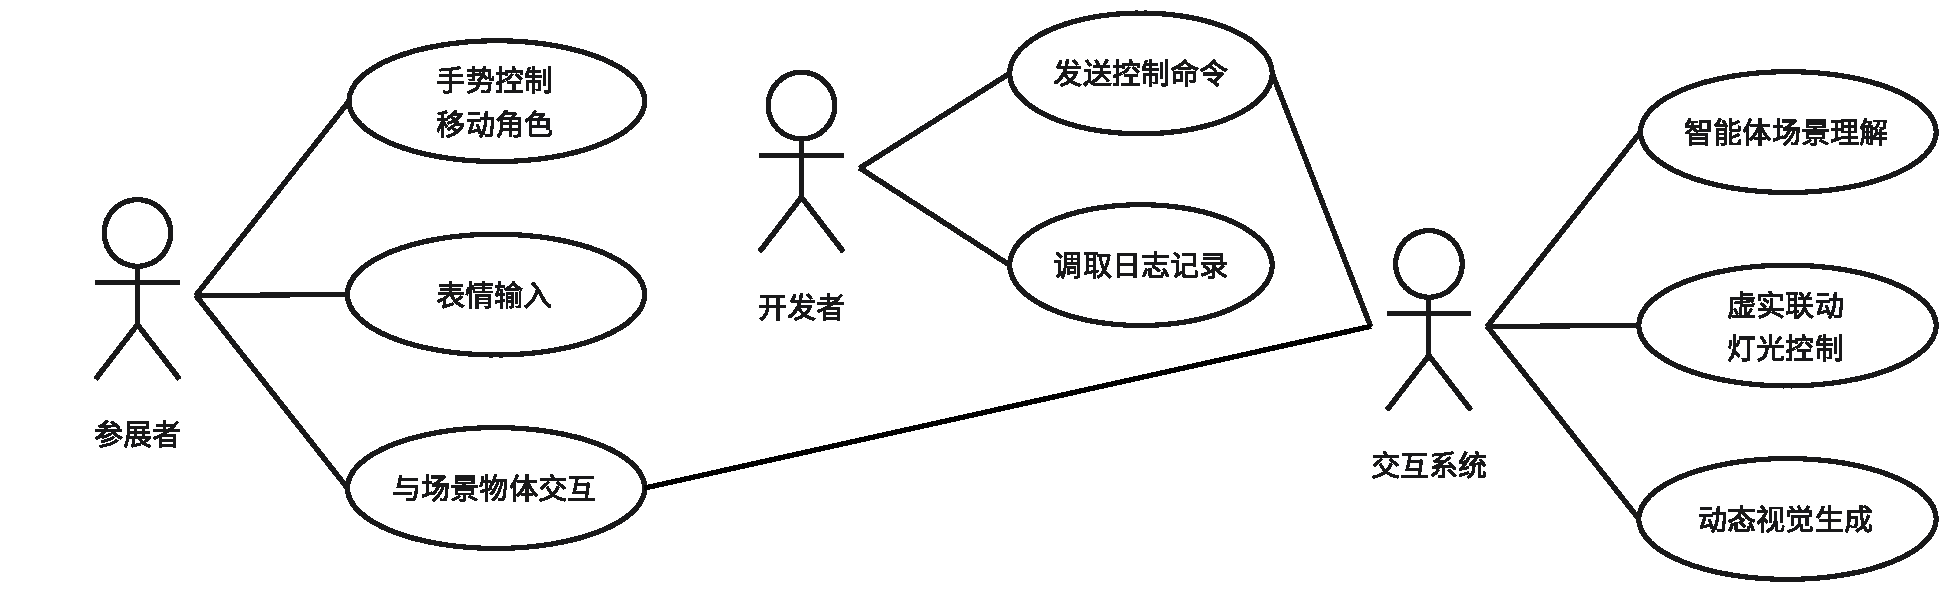
\includegraphics[width=1.0\textwidth]{pic/毕设用例图.pdf}
  \caption{交互系统功能用例图}
  \label{fig:use-case}
\end{figure}

(1) 手势控制移动角色

首先介绍手势交互控制旅人移动的用例。在人们日常生活中，手势往往是语言以外高效的信息传递方式——点名、问路时人们会下意识地用手指向所指代的物体，”所指”一词本身就包含了”指”这个字。因此，为发挥实体展览身体在场性的优势，手势输入必不可少。通过手指指向控制旅人行走，能够达成非常直观的交互感受。系统应在参展者食指伸直时，识别食指所指方向，并控制旅人沿此方向行走。其用例结构化描述如表\ref{tbl:usecase-gesture}所示。

\begin{table}[h]
\centering
\caption{手势交互控制角色移动用例结构化描述}
\begin{tabularx}{\linewidth}{|c|X|}
\hline
Actors & 参展者、MediaPipe模块、Unity \\
\hline
Trigger & 参展者伸直食指指向某一方向 \\
\hline
Preconditions & 各模块已启动并处于正常工作状态，Unity交互应用处于可自由移动模式 \\
\hline
Description & 参展者伸出食指指向目标方向；系统识别指向手势并解析所指方向；旅人角色沿参展者所指方向持续行走；摄像机平滑跟随角色移动 \\
\hline
Postconditions & 旅人角色位置持续更新至参展者所指方向 \\
\hline
Notes & 移动速度恒定，方向随手势连续变化实时更新；仅当食指伸直且其余四指弯曲时识别为指向手势；手势识别到角色响应的端到端延迟在100ms以内 \\
\hline
\end{tabularx}
\label{tbl:usecase-gesture}
\end{table}

(2) 表情输入

手势提供了空间指向性，而面部表情则承载了参展者的情绪信息。系统通过摄像头实时采集参展者的面部图像，持续捕获其自然表情变化；当表情发生显著变化时，系统将面部状态数据上报至EchoAgent，为后续决策提供情感上下文。此过程不涉及参展者的主动交互触发，属于后台持续运行的数据采集链路，其用例描述如表\ref{tbl:usecase-expression}所示。

\begin{table}[h]
\centering
\caption{表情输入用例结构化描述}
\begin{tabularx}{\linewidth}{|c|X|}
\hline
Actors & 参展者、MediaPipe面部识别模块、EchoAgent \\
\hline
Trigger & 参展者面部处于摄像头视野内 \\
\hline
Preconditions & 摄像头与面部识别模块已初始化并正常工作 \\
\hline
Description & 参展者面部处于摄像头视野内，其自然表情变化被持续捕获；当表情发生显著变化时，系统将面部状态数据上报至EchoAgent；Agent据此更新对参展者当前情绪状态的内部表征 \\
\hline
Postconditions & Agent获得参展者当前面部状态数据，更新内部情感上下文 \\
\hline
Notes & 面部检测帧率不低于15fps；仅当表情变化幅度超过阈值且距上次上报超过最小间隔时才触发上报，避免频繁无效推送；情绪分类的语义理解由Agent完成 \\
\hline
\end{tabularx}
\label{tbl:usecase-expression}
\end{table}

(3) 与场景物体交互

前述两项用例关注外部感知输入，而交互应用内部的物体交互构成了叙事推进的核心机制。参展者通过手势引导旅人接近场景中的可交互物体——收集音符以解锁章节进度、激活机关以改变场景结构、触发叙事事件以推进情感故事线。关键交互事件同步通知EchoAgent，使Agent感知参展者的叙事进度。其用例描述如表\ref{tbl:usecase-interaction}所示。

\begin{table}[h]
\centering
\caption{与场景物体交互用例结构化描述}
\begin{tabularx}{\linewidth}{|c|X|}
\hline
Actors & 参展者、Unity交互应用、EchoAgent \\
\hline
Trigger & 参展者控制旅人角色进入场景中可交互物体的触发范围 \\
\hline
Preconditions & Unity交互应用正常运行，旅人角色处于可移动状态，场景物体已加载 \\
\hline
Description & 参展者引导旅人接近场景中的可交互物体（音符、触发器、叙事标记点）；系统检测角色与物体接触后触发对应的交互效果——收集音符、激活机关或触发叙事事件；场景状态与交互进度随之更新；关键交互事件同步通知EchoAgent \\
\hline
Postconditions & 场景交互状态更新，叙事进度推进至下一里程碑 \\
\hline
Notes & 不同物体触发不同的交互效果，所有交互事件通过统一通道通知Agent \\
\hline
\end{tabularx}
\label{tbl:usecase-interaction}
\end{table}

(4) 智能体场景理解

上述感知输入——手势指向、表情变化与场景交互事件——最终汇聚至EchoAgent，由Agent完成跨模态的语义整合与意图推理。Agent将多源感知数据与当前叙事状态统一考量，综合判断参展者的行为意图与情感趋向，生成结构化的决策输出。这一用例属于系统内部的处理链路，不涉及参展者的直接交互，却是连接感知与反馈的关键认知桥梁。其用例描述如表\ref{tbl:usecase-understanding}所示。

\begin{table}[h]
\centering
\caption{智能体场景理解用例结构化描述}
\begin{tabularx}{\linewidth}{|c|X|}
\hline
Actors & EchoAgent、MediaPipe模块、Unity交互应用 \\
\hline
Trigger & Agent接收到来自感知层的多源数据更新（手势、表情、场景事件） \\
\hline
Preconditions & 感知层各模块正常运行，Agent通信链路畅通，叙事状态机已初始化 \\
\hline
Description & Agent汇集手势指向、表情变化与场景交互事件等多源信息；综合当前叙事状态进行意图推理与情感判断，评估是否触发状态转移；根据推理结果确定交互策略——调整场景视觉参数、切换灯光氛围或推进叙事状态；生成结构化的决策输出供执行端使用 \\
\hline
Postconditions & Agent完成场景状态理解，生成决策输出（目标视觉参数、灯光模式、叙事状态更新） \\
\hline
Notes & Agent基于VLM的视觉--语言联合推理完成多模态理解；内部保留近期关键交互历史作为上下文 \\
\hline
\end{tabularx}
\label{tbl:usecase-understanding}
\end{table}

(5) 发送控制命令

Agent完成场景理解与决策后，需将决策结果转化为各执行端可解析的控制指令。指令分别下发至Unity交互应用与灯光控制器，Unity据此更新场景渲染参数与叙事状态，灯光控制器据此更新实体灯阵的模式与颜色，各执行端确认指令执行完毕。其用例描述如表\ref{tbl:usecase-command}所示。

\begin{table}[h]
\centering
\caption{发送控制命令用例结构化描述}
\begin{tabularx}{\linewidth}{|c|X|}
\hline
Actors & EchoAgent、Unity交互应用、树莓派灯光控制器 \\
\hline
Trigger & Agent生成决策输出，需要向执行端下发指令 \\
\hline
Preconditions & Agent与各执行端通信链路正常，决策输出已生成 \\
\hline
Description & Agent将决策结果转化为各执行端可解析的控制指令；指令分别下发至Unity与灯光控制器；Unity据此更新场景渲染参数与叙事状态；灯光控制器据此更新LED灯阵的模式与颜色；各执行端确认指令执行完毕 \\
\hline
Postconditions & Unity场景状态与灯光控制器状态按指令更新，Agent收到执行确认 \\
\hline
Notes & 指令采用统一的结构化格式，各执行端按约定字段解析；若执行端未及时确认，Agent将重试一次；重试失败则记入错误日志 \\
\hline
\end{tabularx}
\label{tbl:usecase-command}
\end{table}

(6) 动态视觉生成

Unity接收Agent下发的视觉参数后，实时驱动虚拟场景的动态视觉呈现。场景中的关键视觉元素——山峦的抖动与固化、建筑的舒展与扭曲、潮水的涨落与光点浮动——随参数变化而动态演变；画面色调与后期效果根据情绪倾向相应调整，使整体氛围与当前情感基调保持一致。所有视觉变化以平滑过渡方式呈现，避免突变造成的视觉割裂。其用例描述如表\ref{tbl:usecase-visual}所示。

\begin{table}[h]
\centering
\caption{动态视觉生成用例结构化描述}
\begin{tabularx}{\linewidth}{|c|X|}
\hline
Actors & Unity交互应用、EchoAgent \\
\hline
Trigger & Unity接收到Agent下发的视觉参数更新指令 \\
\hline
Preconditions & Unity交互应用正常运行，场景资源已加载 \\
\hline
Description & Unity接收Agent下发的视觉参数更新；实时驱动场景视觉元素的动态变化——山峦形变、建筑扭曲、水面波动等；画面色调与后期效果根据情绪倾向相应调整；所有视觉变化以平滑过渡方式呈现，避免突变 \\
\hline
Postconditions & 虚拟场景视觉呈现更新至与当前情绪状态和叙事进度匹配 \\
\hline
Notes & 视觉过渡过程平滑自然，画面帧率保持在可交互水平；场景中各视觉元素的形变幅度与情绪强度正相关 \\
\hline
\end{tabularx}
\label{tbl:usecase-visual}
\end{table}

(7) 虚实联动灯光控制

虚拟场景的视觉变化通过实体LED灯阵延伸至物理展览空间，使沉浸感从屏幕内部扩散至真实环境。Agent根据场景理解结果确定目标灯光模式、颜色与亮度，通过灯光控制器驱动LED灯阵执行对应效果，使实体空间的光影氛围与虚拟场景的视觉基调协调一致。其用例描述如表\ref{tbl:usecase-light}所示。

\begin{table}[h]
\centering
\caption{虚实联动灯光控制用例结构化描述}
\begin{tabularx}{\linewidth}{|c|X|}
\hline
Actors & EchoAgent、树莓派灯光控制器、WS2812 LED灯阵 \\
\hline
Trigger & Agent判定当前场景状态需要灯光氛围变化 \\
\hline
Preconditions & 灯光控制器通信正常，LED灯阵电源接通 \\
\hline
Description & Agent根据场景理解结果确定目标灯光模式、颜色与亮度；灯光控制器接收指令并驱动LED灯阵执行对应效果；实体展览空间的灯光氛围与虚拟场景保持协调一致 \\
\hline
Postconditions & LED灯阵切换至指定灯光模式，实体空间与虚拟场景视觉氛围协调一致 \\
\hline
Notes & 支持追逐、常亮、彩虹渐变、呼吸四种预设灯光模式；灯光变化延迟在200ms以内 \\
\hline
\end{tabularx}
\label{tbl:usecase-light}
\end{table}

(8) 调取日志记录

多模态链路长且包含模型黑盒，系统需内置完善的调试与监控能力。开发者通过专用调试客户端发起日志查询请求，Agent根据指定条件检索运行日志并返回格式化结果，支撑开发阶段的链路追踪与问题定位，也用于展览运行期间的状态监控。其用例描述如表\ref{tbl:usecase-log}所示。

\begin{table}[h]
\centering
\caption{调取日志记录用例结构化描述}
\begin{tabularx}{\linewidth}{|c|X|}
\hline
Actors & 开发者/调试客户端、EchoAgent \\
\hline
Trigger & 开发者通过调试客户端发起日志查询请求 \\
\hline
Preconditions & 系统运行中，日志模块正常工作，调试客户端与Agent通信正常 \\
\hline
Description & 开发者通过调试客户端发起日志查询，指定时间范围、模块与日志级别；Agent检索匹配的运行日志并返回格式化结果；开发者基于日志进行链路追踪、问题定位或状态监控 \\
\hline
Postconditions & 开发者获取指定范围的系统运行日志 \\
\hline
Notes & 日志按模块和时间戳索引；支持按级别过滤与关键词模糊搜索 \\
\hline
\end{tabularx}
\label{tbl:usecase-log}
\end{table}

\section{媒体形式与交互设计理念}

\subsection{立题立意}

《回声之境》以叙事性交互为核心特征，伴随参展者情绪变化与章节推进，在不同阶段营造差异化的场景情绪基调。各场景内，旅人的音符音色、音阶与背景音乐的调式保持和声协调，力求营造富有诗意的沉浸式参观体验。

场景情绪基调：

叙事结构与手法方面，《回声之境》以旅人的旅程为叙事主线，隐喻个体从自我迷茫走向全然自由的成长历程，围绕自我认知、人际边界与知识接纳三层命题展开。交互应用依此设置三个章节——初域·未定之原、聚落群·彼方的光影之城、深流之径·未被触及的知识海——三者在情感基调与交互机制上层层递进。

\subsection{交互场景与引导}

基于上述三章叙事结构，本系统为各章设计了对应的交互场景与关卡流程，确保情感叙事与交互机制深度融合。如表\ref{tbl:chapter-emotion}所示，三章分别对应“迷茫—锚定”“碰撞—边界”“敬畏—自由”三组情感状态的转换，各章的解锁目标、核心交互机制与视觉意象形成一一映射关系。

\begin{table}[h]
\centering
\caption{三章情感状态与交互设计映射}
\begin{tabularx}{\linewidth}{|c|c|c|c|X|}
\hline
\textbf{章节} & \textbf{情感转换} & \textbf{解锁音符} & \textbf{核心机制} & \textbf{视觉意象} \\
\hline
初域·未定之原 & 迷茫→锚定 & 水滴 & 固化流动元素 & 半透明抖动山峦逐渐坚实 \\
\hline
聚落群·光影之城 & 碰撞→边界 & 道路交错 & 情绪折射与共鸣 & 建筑随情绪舒展或扭曲 \\
\hline
深流之径·知识海 & 敬畏→自由 & 海浪、风 & 知识潮渐进机制 & 潮水涨落与深渊光点 \\
\hline
\end{tabularx}
\label{tbl:chapter-emotion}
\end{table}

\subsubsection*{第一章：初域·未定之原——自我迷茫与锚定}

本章对应情感状态从“迷茫”到“锚定”的转换，核心目标是引导参展者解锁水滴音符，学会在未定中锚定自我。设计理念借鉴《最后的篝火》的温柔引导机制：全程无惩罚，通过渐进式教学使参展者理解“我的声音可以塑造世界”的核心逻辑。

远景山峦在本章中承担视觉引导与情感暗示的双重职责。半透明、边缘模糊的山峦形态隐喻旅人尚未明晰的方向感——山体的不稳定抖动象征内心的徘徊与探寻；当山峦被音符固化后逐渐变得坚实，则对应旅人在迷茫中逐步锚定自我、找到方向的过程。视觉层面的虚实转换与情感层面的迷茫-锚定转变形成对照，使参展者在潜意识层面感受情绪叙事的递进。

关卡流程依循四个递进阶段展开：参展者首先从迷雾中显现，面对半透明流动的山峦与旷野，在旁白引导下尝试与世界互动；随后在引导下奏响水滴音符，山峦短暂抖动后恢复流动，参展者需持续奏响以完成固化；继而进入三个方向锚点谜题——“落定的石阶“（过去的锚点）要求参展者观察漂浮石块的流动规律并在恰当时机固化，”无风的山谷“（当下的锚点）需依次固化乱流核心以平息环境扰动，”迷雾的边界“（未来的锚点）则要求参展者自主判断固化的位置与方向，独立开辟道路。三个锚点全部激活后，迷雾散去，未定之原固化为稳定地貌，一条宽阔光路延伸向下一章节。

本章多模态交互涵盖四个维度：持续捏合手势映射为持续奏响音符；发声音量控制固化范围；山体从半透明流动态渐变为坚实青翠形态；水滴音符从单音发展为完整旋律短句。

\subsubsection*{第二章：聚落群·彼方的光影之城——关系探索与边界}

本章对应情感状态从“碰撞”到“边界”的转换，核心目标是解锁道路交错音符，使参展者学会在关系中保持自我边界。设计理念参考《最后的篝火》“中心枢纽+多分支故事线”结构，四个分支区域各自对应一段社交与情感的隐喻。

旅人进入城市时，嘈杂人声导致街道挤压变窄，尝试以水滴音符应对无效——系统由此暗示旧规则在此失效，需要习得新的交互能力。关卡设置四个分支区域：“回声交汇所”中，参展者帮助影子旅者连接断裂的光路，通过动作同步建立共鸣后用水滴音符连接彼此道路；“情绪风塔”中，参展者逐层应对欢喜、悲伤、愤怒、恐惧四种情绪，在共情与自我保护之间寻找平衡；“镜影回廊”中，参展者在布满镜面的空间里忽略扭曲的影像评价，锚定真实的自我；“离别的岔路口”中，参展者帮助影子旅者理解离别并非终结，各自走向属于自己的方向。集齐四个分支的碎片后，城市建筑停止挤压变形，旅人脚下的道路恢复宽阔平稳。

本章引入三项核心交互机制：情绪折射——建筑形态随旅人情绪强度变化，情绪平静时建筑舒展，波动时则扭曲挤压；共鸣系统——与影子旅者的动作同步率达到阈值后触发共鸣效果；边界保护——道路交错音符可在参展者周围划定视觉化的自我边界，过滤外界情绪的干扰。

\subsubsection*{第三章：深流之径·未被触及的知识海——知识接纳与自由}

本章对应情感状态从“敬畏”到“驾驭”再到“自由”的多阶段转换，核心目标是依次解锁海浪音符与风音符，使参展者获得完全的表达自由。设计理念围绕“学得越多，未知越多”的核心命题展开，通过知识潮机制实现渐进式挑战。

关卡分为浅滩区与深潮区两个阶段。浅滩区引入知识潮机制：参展者每获取一个知识碎片（依次对应观察、耐心、试错、联结、放下、接纳六项学习特质），潮水便上涨一层，可立足的礁石减少，但深渊中的光点更加明亮密集。集齐六个碎片后解锁海浪音符，参展者由此学会在知识的潮水中保持稳定。深潮区设置三道情感浪潮，分别对应迷茫、遗憾、无知三种成长困境，旅人需运用已解锁的音符逐一化解。触碰海心之核后，四个音符的旋律汇聚为一首完整的乐曲，风音符随之解锁——参展者由此获得完全的表达自由。值得提及的是，开篇的晴天娃娃在深潮区回归，旅人由此明白它从未抛下自己，只是在前方等待，在叙事层面形成伏笔回收。

完成深潮区挑战后，系统进入自由探索阶段：参展者可自由奏响四个音符，每个音符均会改变整个世界的视觉形态，实现无限的个性化探索。该阶段使参展者充分体验“学以致用”的成就感与“随心所欲不逾矩”的自由状态。

三章的叙事线索层层递进：第一章聚焦自我认知，未定之原是对自我迷茫的具象化；第二章聚焦关系探索，光影之城是对人际边界的具象化；第三章聚焦世界接纳，深流之径是对知识与未知态度的具象化。四个音符作为锚定自我、连接他人、驾驭未知、通达自由的四重能力象征，共同构成了旅人从迷茫走向自由的完整成长弧线。

\subsubsection{音乐交互设计}

从应用名称《回声之境》可以看出，本设计的初衷是构建一个音乐驱动的互动体验——\textit{an experimental interactive application where sound shapes the world}。基于整体应用的叙事特性，各场景绑定特定的配乐调式与速度标识：不同场景运用不同调式与曲速的背景音乐，旅人演奏的音符若不在当前调式上会造成和声冲突。因此，每个场景均预设固有的调式与曲速标识，该设计参考了游戏《Songbird Symphony》中的音乐交互机制。

旅人在旅程中可依次获得四个音符。音符不仅是演奏与视觉反馈的载体，更是旅人理解世界、塑造世界的方式。每个音符承载着隐喻性的象征意义，其演奏效果对应精神层面的某种能力，如表\ref{tbl:note-design}所示。

\begin{table}[h]
\centering
\caption{音符设计表}
\begin{tabularx}{\linewidth}{|c|c|X|}
\hline
音符名称 & 英文名 & 演奏效果与象征意义 \\
\hline
水滴 & waterdrop & 奏响它，可让流动、未定的世界元素固化成型，为自己锚定前行的路标。 \\
\hline
道路交错 & crossing & 奏响它，可与他人的灵魂产生共鸣，连接彼此的道路；也可划定自己的边界，让自己不受他人情绪与评价的影响。 \\
\hline
海浪 & tide & 奏响它，可驾驭知识的潮水，让流动的未知成为你前行的路；也可让你在潮水里保持稳定，不被洪流吞噬。 \\
\hline
风 & breeze & 奏响它，可让你的声音传遍整个回声之境，你走过的路，会成为后来者的路标；你也可以化作风，去往任何你想去的地方，无拘无束。 \\
\hline
\end{tabularx}
\label{tbl:note-design}
\end{table}

上述四个音符的设计层层递进，映射了旅人从认识自我、到处理与他人关系、再到汲取知识、最终获得自由的成长路径。在交互应用进程中，四个音符通过指引依次获得——这既是叙事节奏的安排，也隐喻着人生中认知与能力逐步展开的顺序。音符的演奏将触发不同的视觉与音效反馈，同时驱动场景元素的动态变化，使音乐真正成为塑造交互应用世界面貌的核心力量。


\subsubsection{多模态展览适配}

为适配实体展览的公共交互场景，系统在交互机制层面做了以下针对性设计。

\textbf{无惩罚机制}：全程不设失败判定与进度回滚，参展者未完成谜题时仅返回入口重新尝试。系统不会施加负面反馈，仅静待参展者找到解法，给予充分的安全感与试错空间。

\textbf{轻量化操作}：核心交互仅包含移动与四个音符的演奏，无需复杂连招或精确时序操作，适配全年龄段的参观者群体。

此外，所有交互机制均设计为多模态兼容，支持虚拟端（键盘、鼠标、触摸屏）与实体端（手势、麦克风、实体按钮）的双轨输入，并在两种模式下保持视觉、音频与灯光反馈的协调一致，如表\ref{tbl:multimodal-adaptation}所示。

\begin{table}[h]
\centering
\caption{多模态交互适配表}
\begin{tabularx}{\linewidth}{|c|c|c|c|}
\hline
\textbf{交互类型} & \textbf{虚拟交互} & \textbf{实体展览交互} & \textbf{反馈协调} \\
\hline
音符演奏 & 按键/触摸屏 & 体感手势/麦克风发声 & 视觉+音频+灯光同步 \\
\hline
移动控制 & 键盘/手柄 & 体感移动/地面投影 & 摄像机跟随+场景变化 \\
\hline
情绪感知 & 应用内情绪值 & 面部识别/心率传感 & 自适应参数调整 \\
\hline
环境交互 & 鼠标点击 & 触摸大屏/实体按钮 & 多感官协调反馈 \\
\hline
\end{tabularx}
\label{tbl:multimodal-adaptation}
\end{table}

这种章节递进与多模态适配相结合的设计，使《回声之境》不仅是一个交互应用，更是一段完整的情感成长旅程——参展者在解锁音符、破解谜题的过程中，经历从自我迷茫到全然自由的情感蜕变。


\subsection{旅人人物形象设计}

\textbf{「那位没有过去，却正被未来召唤的人」}

没有人知道旅人从何而来。当他睁开眼时，正立于“未定之原”的浅雾中，风声像未完成的句子，光像正在犹豫的记忆。他没有名字，不是因为遗忘，而是因为他从未真正拥有过。旅人不是被放逐，也不是被召唤——他之所以存在，是因为回声之境“正在形成”，而只有那些心中仍在寻找自我形状的人，才会在世界未成形之时走进它。

在他胸口，有一块微弱跳动的光核——不是心脏，而是他尚未理解的自己。随着他前行，光会改变颜色、节奏与温度：它既是力量，又是负担；既是答案，又是疑问本身。旅人来到这里，是因为他已走到人生某个模糊的分叉——不再属于过去，却尚未准备好面对未来。回声之境正是这种状态的具象化。因此，旅人不是外来的闯入者，而是这个世界尚未成形部分的化身。

\section{总体架构和通信协议}

\subsection{系统总体架构}

以上述设计原则为指导，本系统最终形成了如图\ref{fig:system-arch}所示的三层星型拓扑架构。图\ref{fig:tech-roadmap}展示了开题阶段规划的技术路线，为架构设计提供了方法论基础。

\begin{figure}[htbp]
  \centering
  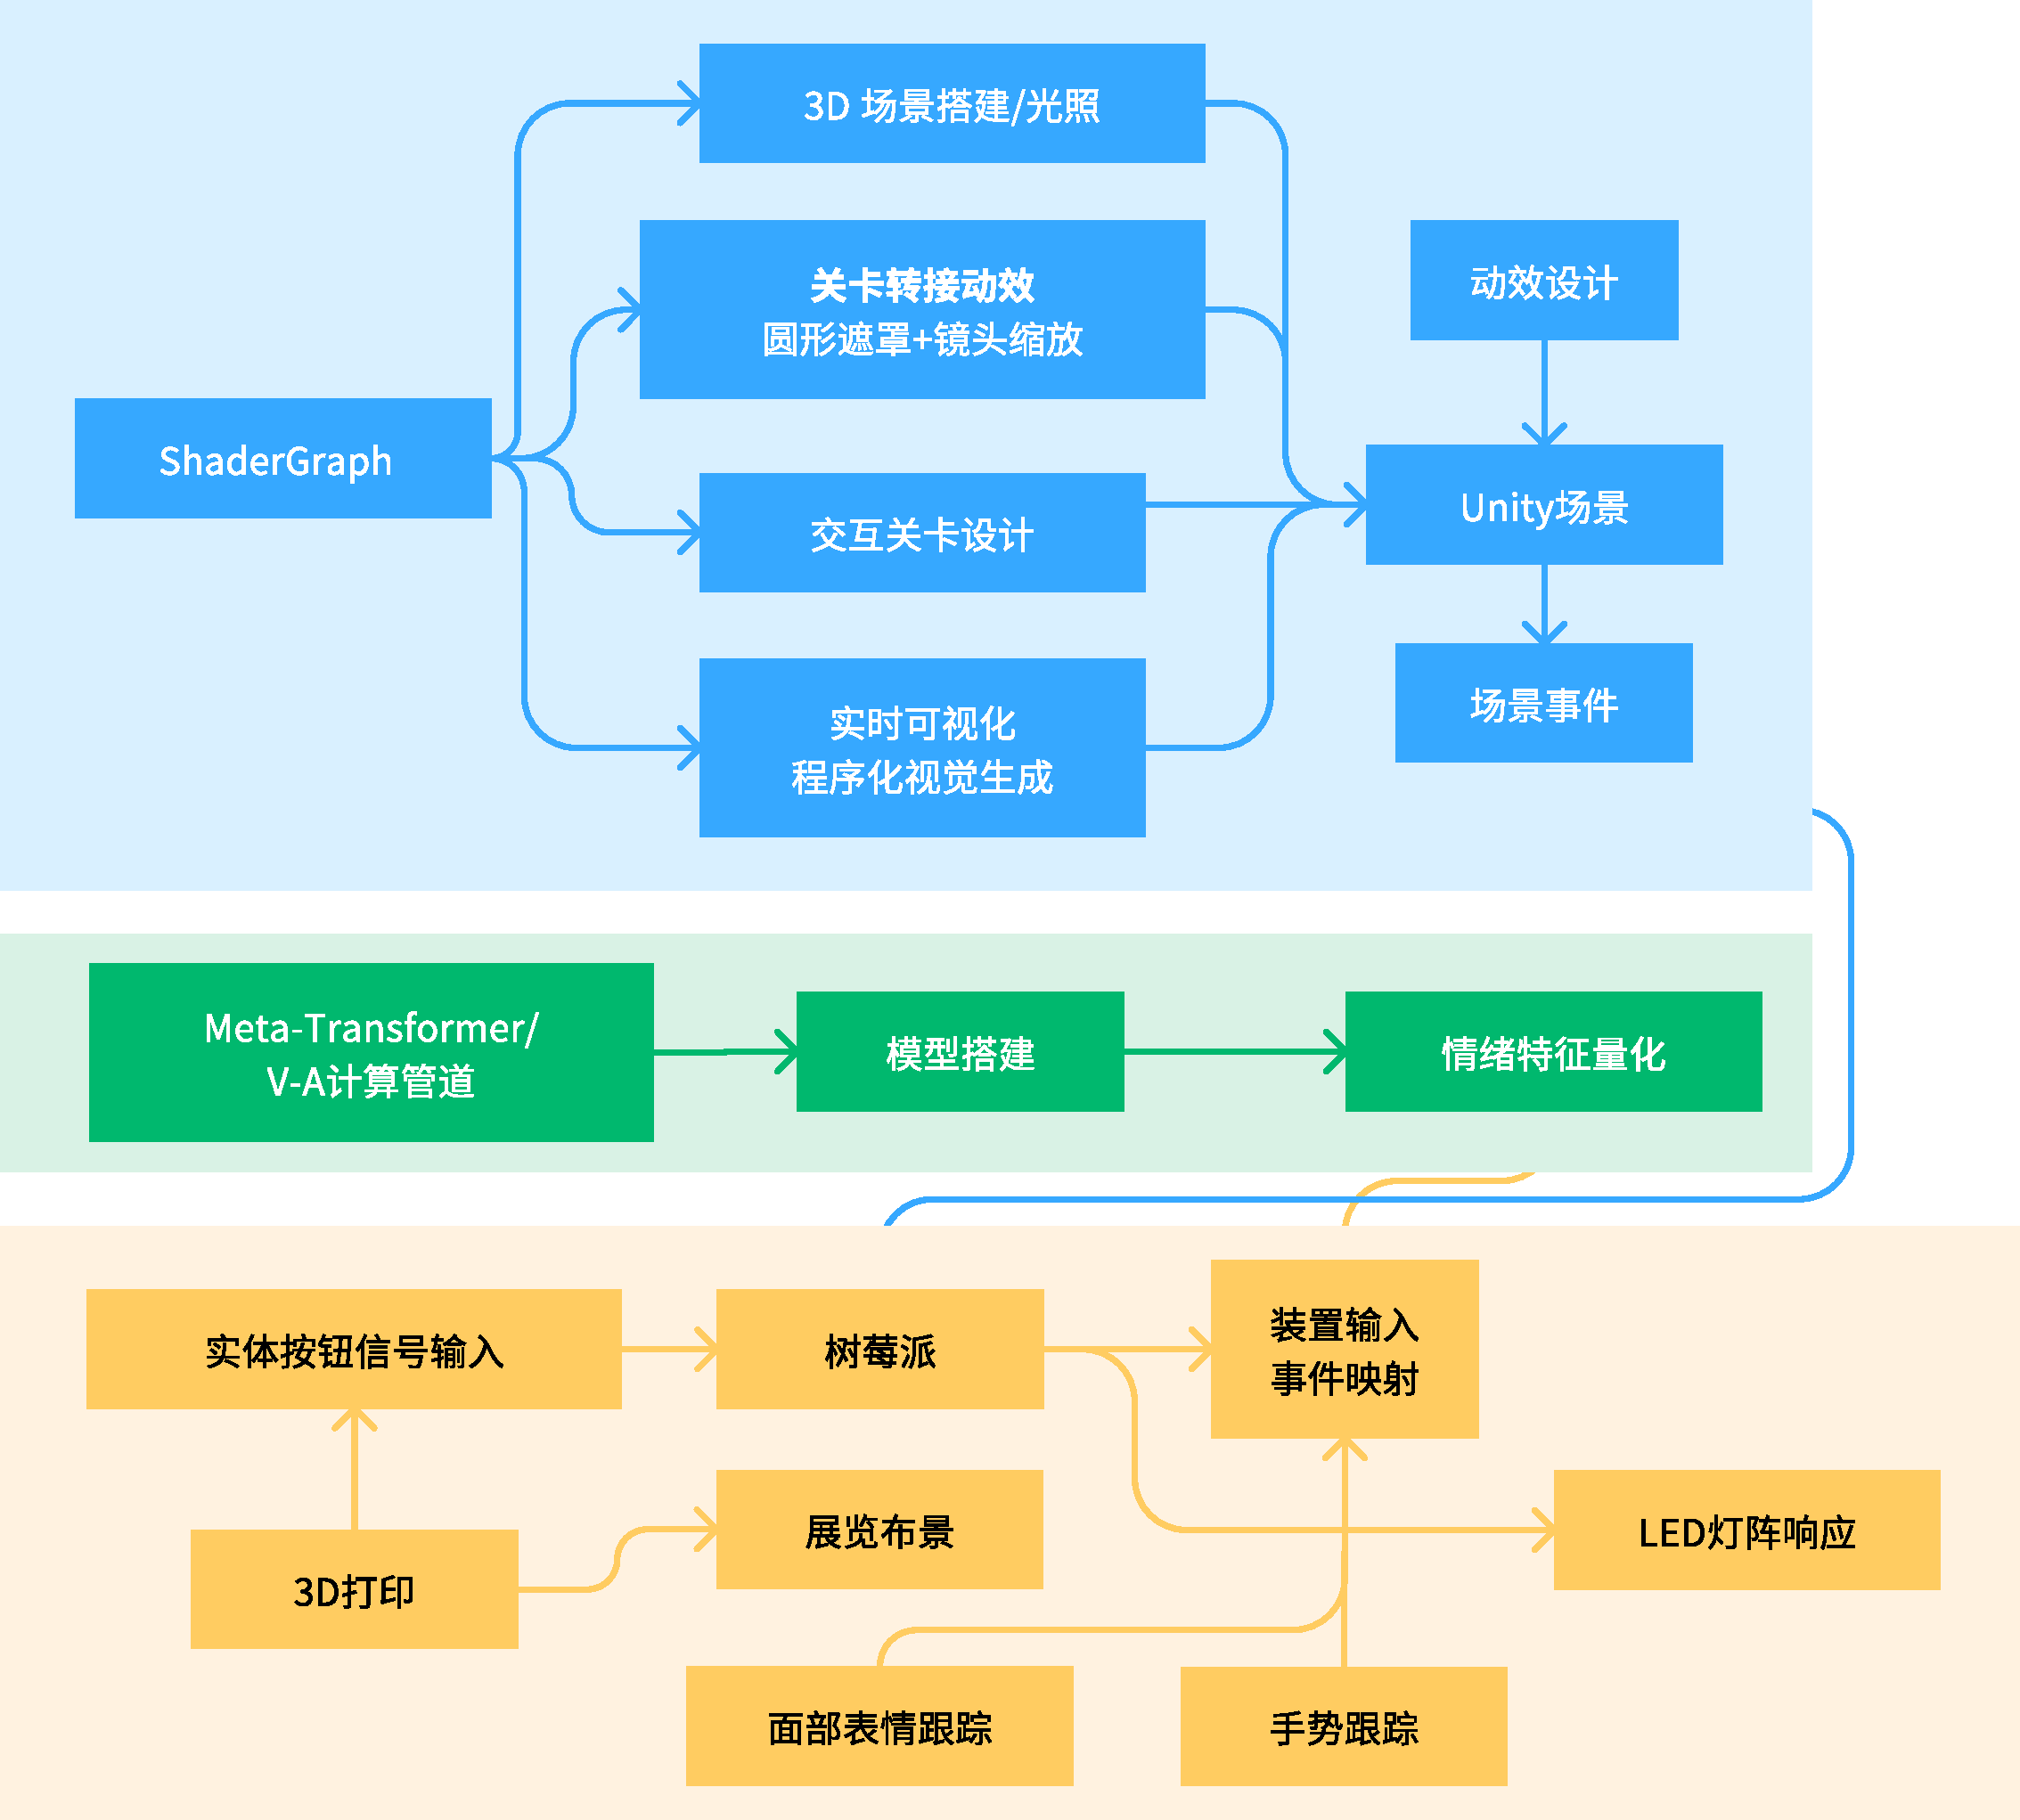
\includegraphics[width=0.9\textwidth]{pic/开题报告技术路线图.pdf}
  \caption{技术路线图}
  \label{fig:tech-roadmap}
\end{figure}

\begin{figure}[htbp]
  \centering
  \includegraphics[width=0.9\textwidth]{pic/面向实体展览的沉浸式多模态交互系统 架构图.pdf}
  \caption{系统总体架构图}
  \label{fig:system-arch}
\end{figure}

如图\ref{fig:system-arch}所示，本系统采用“感知层—理解层—反馈层”的三层星型拓扑架构。

\textbf{感知层}由四个独立模块构成：MediaPipe手势识别模块负责检测参展者的手部动作（捏合、滑动、指向等）；面部情绪识别模块实时分析参展者的情感状态；Unity交互应用同步上报当前章节进度与场景事件；摄像头则提供原始视觉输入。各模块均以TCP Client方式将感知数据上报至理解层，体现了全流程多模态的设计原则——手势、表情、应用状态三类异构信息统一汇入决策中枢，而非各自独立处理。

\textbf{理解层}以EchoAgent为核心。EchoAgent内部基于大语言模型构建，结合DeepAgent框架实现Tool Calling能力，统一汇聚多源感知信息并综合推理，生成针对性的控制指令。EchoAgent与TCP Server之间通过消息队列解耦：Server负责网络通信，将接收到的客户端消息投入共享队列；EchoAgent则按固定间隔从队列中取出消息，经大语言模型理解后自主决策并调用相应工具。这种设计使决策逻辑与网络通信完全分离——EchoAgent并非TCP客户端，而是通过内部队列与Server协同，Server专注收发，Agent专注推理，二者各司其职。

\textbf{反馈层}由Unity客户端与树莓派物理装置组成，分别承担虚拟场景渲染与实体灯光控制任务。这一双层反馈结构是虚实结合设计原则的直接体现：同一决策指令可同时驱动虚拟画面变化与物理灯光响应，使展览交互从屏幕内延伸至实体空间，形成完整的“感知—理解—反馈”闭环。

系统采用TCP/IP协议实现模块间通信。TCP Server作为通信中枢，接收来自各感知模块的数据上报，并将决策指令下发至反馈模块。Unity客户端、MediaPipe客户端、树莓派客户端及调试客户端均作为TCP Client连接至决策中枢，共同构成星型拓扑结构。这种结构实现了各模块的松耦合：各感知模块仅需关注自身数据采集，无需了解其他模块的存在；决策模块则充当统一的信息汇聚与分发中心，协调各模块间的数据流转，充分体现了强可拓展性原则——新增感知通道或反馈设备只需以TCP Client接入，无需修改核心决策逻辑。

在通信协议的选择上，本系统经过深入比较，最终确定采用TCP Socket而非WebSocket作为传输层协议。TCP Socket相比WebSocket具有更低的协议开销和传输延迟，且能够提供更精细的流量控制与连接管理能力，便于针对展览场景的特定需求进行优化调参。

\subsection{自定义TCP通信协议}

在协议格式的设计过程中，本系统经历了从二进制协议到JSON文本协议的演进历程。

\textbf{（1）二进制协议方案}：早期设计采用长度前缀结合消息类型的二进制协议格式，具体结构为：4字节大端序无符号整数表示载荷长度，1字节无符号整数表示消息类型（\texttt{0x00=TEXT}、\texttt{0x01=IMAGE}、\texttt{0x02=COMMAND}、\texttt{0x03=REGISTER}），其后为载荷数据。该方案在理论上具有最高的解析效率，但在实际开发中暴露出两个问题：其一，图片数据与文本数据采用完全不同的编码路径，处理混合类型消息时需要额外的类型判断与解码逻辑，增加了开发复杂度；其二，二进制格式无法在开发阶段直接阅读，调试与问题定位均较为困难。

\textbf{（2）JSON文本协议方案}：基于上述实践经验，本系统最终采用“4字节大端序长度前缀 + UTF-8编码JSON载荷”的协议格式。发送端将JSON对象序列化为UTF-8字节序列，计算其长度并以大端序写入前4字节，随后写入载荷；接收端据此解析，确保TCP流式传输中消息边界的正确划分。该协议将所有数据统一封装为JSON对象，核心字段定义如下：

\begin{itemize}
\item \texttt{type}：消息类型，取值为 \texttt{text}（普通文本消息）、\texttt{image}（Base64编码的图片数据）、\texttt{command}（控制命令）、\texttt{register}（客户端注册）
\item \texttt{data}：载荷内容——文本消息时为UTF-8字符串，图片消息时为Base64编码的二进制数据，command类型时为具体命令名称
\item \texttt{client\_type}：发送者身份标识，取值包括 \texttt{unity}、\texttt{mediapipe}、\texttt{raspberry\_pi}、\texttt{debug} 四种。客户端在注册时通过此字段声明自身类别，服务端据此维护已连接客户端的注册表
\item \texttt{request\_id}：请求追踪标识，采用UUID格式。当命令需要响应时，发起方携带此字段，响应方须原样回传以关联请求—响应对
\item \texttt{relay\_to}：直接转发标识。若消息中包含此字段，服务端不再将消息投入Agent队列，而是直接转发至目标客户端，实现低延迟的客户端间直连通信
\end{itemize}

其中，\texttt{register}类型具有特定的语义约定：该类型仅由客户端向服务端发起。当客户端首次连接到服务端时，须发送一条\texttt{register}类型消息并携带\texttt{client\_type}字段标识自身类别。服务端在收到注册消息后记录该连接的身份信息，后续该连接发送的消息无需重复携带\texttt{client\_type}，服务端将自动补充发送者身份。

JSON文本协议具有三方面优势：文本形式便于开发阶段的调试与日志分析；统一的数据封装方式简化了协议解析逻辑；Base64编码虽然增加了约33\%的数据体积，但换取了协议的一致性与可维护性。考虑到本系统运行于本机与局域网环境下，网络带宽充足且延迟极低（通常低于5ms），上述开销在实际使用中完全可接受。表\ref{tbl:protocol-examples}按消息类型给出了四种典型场景下的协议使用实例。

\begin{table}[h]
\centering
\caption{协议使用实例}
\begin{tabularx}{\linewidth}{|l|X|}
\hline
场景 & 消息格式 \\
\hline
客户端注册 & \texttt{\{"type": "register", "client\_type": "mediapipe"\}} \\
\hline
Unity上报交互应用状态 & \texttt{\{"type": "text", "client\_type": "unity", "data": "chapter:2, event:enter\_scene"\}} \\
\hline
截图响应（带请求追踪） & \texttt{\{"type": "image", "client\_type": "unity", "data": "base64...", "request\_id": "uuid-xxx"\}} \\
\hline
客户端间直接转发 & \texttt{\{"type": "text", "client\_type": "mediapipe", "data": "hand\_pos:0.5,0.3", "relay\_to": "unity"\}} \\
\hline
\end{tabularx}
\label{tbl:protocol-examples}
\end{table}

\subsection{控制命令设计}

基于上述协议格式，系统定义了一套控制命令用于各模块间的协调交互。表\ref{tbl:command-table}按接收客户端分组，汇总了全部控制命令的发起方、接收方与使用说明。

命令的命名遵循三级约定，以前缀区分语义类别：

\begin{enumerate}
\item \textbf{\texttt{request:}前缀}：请求型命令，期望接收方处理后返回响应。发起方须携带\texttt{request\_id}字段，接收方响应时原样回传以关联请求。典型实例为\texttt{request:screenshot}——Agent请求Unity或MediaPipe客户端截取当前画面以查看运行状态。
\item \textbf{\texttt{input:}前缀}：输入注入型命令，用于向目标客户端模拟用户交互事件。典型实例包括\texttt{input:submit}（触发提交事件）、\texttt{input:move}（将食指指向映射为输入坐标）、\texttt{input:cancel}（取消当前输入）和\texttt{input:navigate}（触发导航操作）。
\item \textbf{无前缀}：直接控制命令，即发即忘，无需响应。此类命令主要用于设备控制与状态同步，如灯光模式切换（\texttt{chase}、\texttt{solid}、\texttt{rainbow}、\texttt{breathing}）、音符事件的灯光伴随反馈（\texttt{gain\_note}、\texttt{drop\_note}、\texttt{play\_note}），以及配置开关（\texttt{hand\_direction}）。
\end{enumerate}

\begin{table}[h]
\centering
\caption{系统控制命令汇总}
\begin{tabularx}{\linewidth}{|l|c|c|X|}
\hline
命令名称 & 接收客户端 & 发起客户端 & 使用说明 \\
\hline
\texttt{hand\_direction} & mediapipe & unity & 开关手指方向识别与信息发送 \\
\hline
\texttt{input:submit} & unity & mediapipe & 演示中用于驱散标题文字 \\
\hline
\texttt{input:move} & unity & mediapipe & 识别食指指向，在Unity端映射为输入设备坐标 \\
\hline
\texttt{input:cancel} & unity & echoagent, mediapipe & 取消当前输入操作 \\
\hline
\texttt{input:navigate} & unity & echoagent & 智能体主动触发导航操作 \\
\hline
\texttt{request:screenshot} & unity, mediapipe & echoagent & 智能体主动请求客户端截图以查看当前状态 \\
\hline
\texttt{chase} & raspberry\_pi & debug & 控制灯光为循环点亮模式 \\
\hline
\texttt{solid} & raspberry\_pi & debug & 控制灯光为实色模式 \\
\hline
\texttt{rainbow} & raspberry\_pi & debug & 控制灯光为彩虹渐变模式 \\
\hline
\texttt{breathing} & raspberry\_pi & debug & 控制灯光为呼吸渐变模式 \\
\hline
\texttt{gain\_note} & raspberry\_pi & unity & Unity中触发事件时灯条同步反馈 \\
\hline
\texttt{drop\_note} & raspberry\_pi & debug & 调试用，模拟失去音符时的灯光反馈 \\
\hline
\texttt{play\_note} & raspberry\_pi & unity & 演奏音符时的灯光伴随效果 \\
\hline
\end{tabularx}
\label{tbl:command-table}
\end{table}

从表\ref{tbl:command-table}可见，命令体系完整覆盖了四类客户端之间的交互需求：MediaPipe与Unity之间通过\texttt{input:}前缀命令实现手势到输入的映射；EchoAgent通过\texttt{request:screenshot}主动感知系统运行状态，并通过\texttt{input:cancel}与\texttt{input:navigate}干预交互流程；灯光控制命令以无前缀的简洁形式直接驱动树莓派；音符反馈命令（\texttt{gain\_note}、\texttt{drop\_note}、\texttt{play\_note}）则实现了Unity虚拟事件到物理灯光的实时联动。

\subsection{实体展览环境设计}

实体装置旨在将虚拟世界的交互状态延伸至物理空间，增强观展者的沉浸感与具身参与体验。

\textbf{技能图标实体化}：将交互应用中的四个音符图标实体化，使用椴木板制作展览实物。图标图案采用矢量绘图工具（Affinity Designer）绘制四次贝塞尔曲线构建流畅的音符轮廓线条，经雕刻、镂空处理后配合装饰性麻绳串联固定于展台。实体图标与交互应用内的点亮状态保持同步，当参展者在交互应用中演奏音符时，对应图标同步亮起LED灯效。

\textbf{灯光控制系统}：灯条采用WS2812可编程RGB LED灯带，具有单点可控、色彩丰富、响应速度快的特点。灯带由树莓派通过PWM（脉冲宽度调制）信号控制，树莓派作为TCP Client连接至智能体服务端，接收来自Agent的灯光控制指令（颜色、亮度、闪烁模式），实时驱动灯带产生与虚拟场景同步的动态光影效果。

\textbf{信号传递流程}：实体装置的信号链路为：MediaPipe/Unity感知模块 → TCP上报 → Agent决策 → TCP下发控制指令 → 树莓派PWM驱动LED。树莓派接收到控制指令后，通过Python的rpi-ws281x库将PWM信号转换为LED灯带的显示效果，实现从虚拟场景到实体空间的跨媒介联动。


\chapter{关键技术与模块实现}

\section{智能体EchoAgent实现}

\subsection{运行机制}

EchoAgent 是本系统的理解层中枢，基于大语言模型构建，负责整合多源感知数据并做出交互决策。系统启动时按以下顺序初始化各组件：首先创建一个全局的异步消息队列（\texttt{asyncio.Queue}），随后创建 TCP 服务器（EchoServer）并注入队列引用，最后创建 EchoAgent 实例，使其同时持有队列与服务器的引用。这一初始化顺序确保 Agent 能够通过消息队列接收来自各客户端的上报数据，并通过 EchoServer 向各客户端主动发送指令。

运行时，EchoServer 与 EchoAgent 各自在独立的异步循环中运行。EchoServer 在端口 65432 上持续监听 TCP 连接，接收来自 MediaPipe、Unity 与树莓派等客户端的上报消息，将非注册、非中继类消息写入共享队列。EchoAgent 按固定间隔（默认 5 秒）从队列中批量取出积压消息，交由大语言模型理解与推理，由模型自主选择并调用合适工具完成响应。这种生产者—消费者模式解耦了消息接收与决策处理，使两者可以独立伸缩。

Agent 的完整交互闭环如图~\ref{fig:agent-trace} 所示：MediaPipe 模块检测到参展者的手势或表情变化后，通过 TCP 上报至 Agent；Agent 结合当前叙事章节、参展者进度与情绪上下文进行综合决策，必要时调用截图工具获取 Unity 当前画面以辅助判断；截图请求经 TCP 发送至 Unity 客户端，Unity 执行截图后将图像回传；Agent 理解图像内容后发起下一步交互指令，形成”感知—理解—反馈”闭环。

\begin{figure}[htbp]
\centering
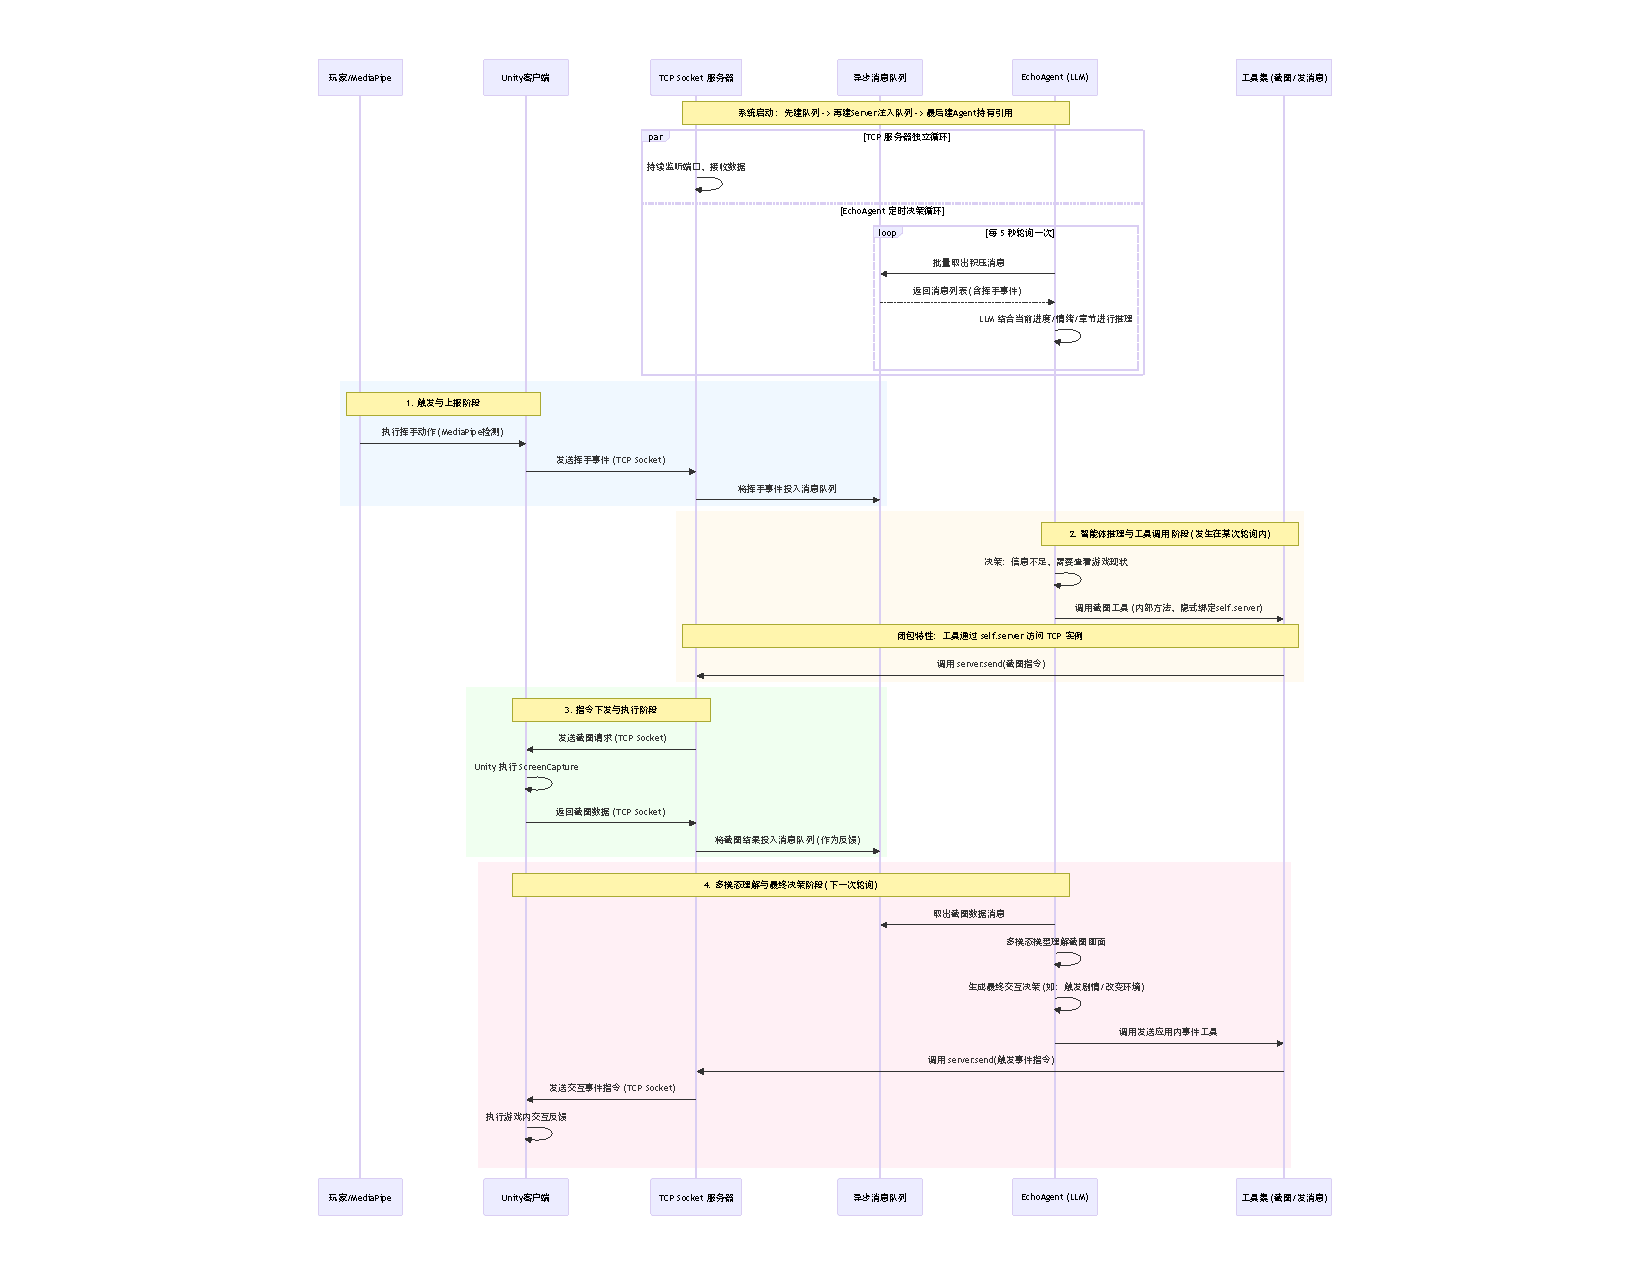
\includegraphics[width=1.0\textwidth]{pic/智能体决策完整流程时序图.pdf}
\caption{智能体决策流程时序图}
\label{fig:agent-trace}
\end{figure}

\subsection{DeepAgent 框架集成}

本系统的 Agent 基于 DeepAgent 框架构建。DeepAgent 是一个基于 LangGraph 与 LangChain 的智能体框架，通过 \texttt{create\_deep\_agent()} 工厂函数创建编译后的状态图（\texttt{CompiledStateGraph}），提供内置的任务规划、上下文管理与子代理委派能力。Agent 使用 \texttt{InMemorySaver} 作为对话检查点存储器，维持跨轮次推理的状态连续性。

在模型接入方面，框架通过 LangChain 的标准 Chat Model 接口与底层大语言模型交互，支持灵活切换模型提供商。系统的系统提示词（System Prompt）通过结构化自然语言向模型传递《回声之境》的交互应用定位、三类客户端角色（Unity、MediaPipe、Raspberry Pi）、消息类型体系（文本与图像），以及关键的调试模式指引——Agent 在收到 Unity 注册消息后主动请求截图以建立场景认知。

\subsection{工具函数设计}

工具调用（Tool Calling）是 Agent 控制外部设备的唯一途径。EchoAgent 通过 LangChain 的 \texttt{@tool} 装饰器定义了五个工具函数，均以 EchoAgent 的静态方法形式实现，在初始化时通过闭包绑定 EchoServer 实例。工具参数均采用简单字符串类型以降低 VLM 生成结构化参数的出错概率：

\begin{enumerate}
\item \textbf{\texttt{send\_to\_client}}：向指定类型的客户端发送通用消息。参数为 \texttt{client\_type}（\texttt{“unity”}、\texttt{“mediapipe”} 或 \texttt{“raspberry\_pi”}）与 \texttt{message}（纯文本）。内部通过 EchoServer 遍历已注册连接，找到匹配类型的客户端后发送 JSON 消息。

\item \textbf{\texttt{request\_unity\_screenshot}}：请求 Unity 客户端截取当前画面并回传。无参数，内部向 Unity 客户端发送 \texttt{request:screenshot} 指令，Unity 端执行截图后以 Base64 编码的 JPEG 图像回传至 Agent，Agent 在下一轮轮询中将其作为多模态上下文的一部分进行分析。

\item \textbf{\texttt{control\_lights}}：控制实体 LED 灯阵。参数为 \texttt{mode}（灯光模式：\texttt{chase} 循环点亮、\texttt{solid} 实色、\texttt{rainbow} 彩虹渐变、\texttt{breathing} 呼吸，以及 \texttt{gain\_note}/\texttt{play\_note} 音符联动反馈）、\texttt{color}（\texttt{solid} 模式的颜色，如 \texttt{warm\_amber}、\texttt{cool\_blue} 等）与 \texttt{note}（音符反馈模式下的音符名称：\texttt{waterdrop}、\texttt{crossing}、\texttt{tide}、\texttt{breeze}）。内部构造 \texttt{lights:mode[:color][:note]} 格式指令，经 TCP 发送至树莓派。

\item \textbf{\texttt{play\_music}}：控制交互应用中的音乐与音频播放。参数 \texttt{action} 为 \texttt{“类别:操作”} 格式字符串——演奏音符（\texttt{play\_note:waterdrop} 等）或切换情绪背景音乐（\texttt{set\_mood:calm/tense/warm}）。内部封装为 \texttt{music:action} 指令发送至 Unity。

\item \textbf{\texttt{speak}}：通过 MiniMax TTS 服务将文本转为语音并播放。参数 \texttt{text} 为待朗读文本。内部调用 MiniMax \texttt{speech-2.8-turbo} 模型，使用 Mandarin Warm Girl 音色生成 MP3 音频并播放。
\end{enumerate}

\subsection{批量消息处理与决策流程}

EchoAgent 的决策循环以轮询模式运行：每 5 秒从消息队列中一次性排空所有积压消息，将其转换为 LangChain 的 \texttt{HumanMessage} 列表后批量送入 Agent。对于文本类消息，直接将原始 JSON 字符串作为消息内容；对于图像类消息，则构造包含 Base64 编码图像与描述文本的多模态内容结构。Agent 通过 \texttt{deep\_agent.ainvoke()} 执行推理，模型根据系统提示词与当前上下文自主决定是否以及调用哪个工具，工具执行结果以 \texttt{ToolMessage} 形式追加至对话历史，供下一轮推理使用。

这种批量处理模式的设计兼顾了两方面考量：一方面，将多源异步到达的消息聚合后统一推理，使 Agent 能够在同一上下文中综合考虑手势、表情与场景事件的关联；另一方面，5 秒的间隔避免了模型 API 的频繁调用，在交互响应性与资源开销之间取得了平衡。

\section{TCP通信与并发控制实现}

\subsection{长度前缀JSON协议}

系统各模块间通过统一的二进制帧协议进行通信：每帧由 4 字节大端序无符号整数（表示负载长度）与紧随其后的 UTF-8 编码 JSON 负载组成。接收方先读取 4 字节长度前缀，再按长度读取完整 JSON 数据，以此实现帧边界划分。JSON 消息体包含以下字段：\texttt{type}（消息类型，可选 \texttt{text}、\texttt{image}、\texttt{command}、\texttt{register}）、\texttt{data}（负载内容）、\texttt{client\_type}（发送方身份标识，注册消息使用）、\texttt{request\_id}（UUID 格式请求标识，用于关联请求与响应）及 \texttt{relay\_to}（中继目标，指定消息经服务器直接转发至某类客户端）。客户端类型包括 \texttt{mediapipe}、\texttt{unity}、\texttt{raspberry\_pi} 与 \texttt{debug}，覆盖系统全部通信节点。

\subsection{EchoServer与客户端管理}

TCP 服务端由 EchoServer 类实现，基于 Python \texttt{asyncio} 在端口 65432 上监听连接。每个客户端连接对应一个 LengthPrefixProtocol 实例，维护独立的接收缓冲区与长度解析状态机。客户端首次连接时须发送注册消息（\texttt{\{"type": "register", "client\_type": "..."\}}），服务端据此将连接与其身份类型绑定，后续的 \texttt{send\_message} 操作遍历已注册连接集合，按类型匹配目标客户端。

协议层支持中继转发机制：若消息含非空 \texttt{relay\_to} 字段，服务端直接将消息转发至匹配类型的所有对等连接，不经消息队列，以此实现客户端间的低延迟直通——典型场景为 MediaPipe 将指向方向数据中继至 Unity 驱动角色移动。不含 \texttt{relay\_to} 的普通消息则写入共享的 \texttt{asyncio.Queue}，交 EchoAgent 处理。

\subsection{Unity端AgentCommunicator}

Unity 侧由 AgentCommunicator 组件（挂载于 GameRoot 持久化对象）承担 TCP 客户端角色。启动时异步连接至 Agent 服务端并发送注册消息，随后在后台 Task 中运行接收循环，按长度前缀协议解析入站消息，根据消息类型分派至对应回调。

在发送侧，\texttt{SendRawAsync} 方法使用 \texttt{SemaphoreSlim(1,1)} 作为发送锁，确保同一时刻仅有一个异步任务持有网络流的写入权，避免多协程并发写入导致的 TCP 数据交错。所接收消息通过 \texttt{SynchronizationContext.Post()} 投递至 Unity 主线程执行回调，符合 Unity 的单线程执行模型。

AgentCommunicator 还负责处理截图请求：当收到 \texttt{request:screenshot} 指令时，在帧末尾调用 \texttt{ScreenCapture.CaptureScreenshotAsTexture()} 获取当前画面，编码为 JPEG 并以 Base64 字符串回传，同时将截图缓存至本地持久化路径供调试使用。

\subsection{调试客户端}

为便于开发阶段的链路追踪与指令模拟，本系统基于 Rust 实现了独立的调试客户端 echo\_client。该客户端提供可编程的 Rust 库（\texttt{EchoClient}），支持基于事件回调（\texttt{on\_text}、\texttt{on\_image}、\texttt{on\_command}）的异步消息订阅，以及 \texttt{send\_text}、\texttt{send\_command}（支持 relay\_to 参数）等发送接口。在此库基础上，通过 warp 框架实现了 WebSocket-to-TCP 桥接服务器（端口 8080），并配套基于浏览器的可视化调试界面——开发者可直接在网页中选择客户端类型、构造消息内容并指定中继目标，实时查看收发日志，极大降低了多模块联调的复杂度。

\section{虚拟场景与视觉呈现}

\subsection{旅人控制器与虚拟输入设备}

旅人角色的移动由 TravelerController 组件驱动，该组件依赖 Unity 的 CharacterController 进行物理位移计算。在 \texttt{FixedUpdate} 中按固定时间步长执行重力施加、输入解析、旋转平滑与位移更新：读取 Input System 的 Move 动作获取二维输入向量，结合主摄像机的偏航角计算世界空间移动方向，通过 \texttt{Mathf.SmoothDampAngle} 实现角色朝向的平滑过渡；垂直方向累计重力加速度，着地时清零。

为使 Agent 能够通过网络指令驱动旅人移动，系统实现了一个自定义的 VirtualAgentDevice——继承自 Unity Input System 的 \texttt{InputDevice}，向 Input System 注册为独立输入设备，提供 \texttt{move\_stick}（二维摇杆）与 \texttt{submit\_button}、\texttt{cancel\_button} 等控制元。EchoEventCenter 组件监听 Agent 下发的 \texttt{input:move:x,y} 格式指令，将解析出的方向向量写入 VirtualAgentDevice 的状态结构，通过 \texttt{InputSystem.QueueStateEvent()} 注入 Input System 事件队列，从而被 TravelerController 的 Move 动作绑定所消费。这一间接层使网络输入与本地键盘/手柄输入共享同一套 Input System 管线，无需在角色控制器中编写特殊的网络输入分支。

为防止 Agent 指令"粘滞"（即上一次移动指令持续生效），EchoEventCenter 内置了移动超时检测：每 0.2 秒检查距最后一次移动指令的时间，若超过 0.3 秒无新指令则自动清零移动向量，使角色在通信中断或 Agent 静默时自动停步。

\subsection{场景物体交互}

场景中的可交互物体通过 IInteractable 接口定义统一契约，包含 \texttt{Interact()}（执行交互逻辑）与 \texttt{GetInteractText()}（返回交互提示文本）两个方法。旅人对象上挂载的 InteractionDetector 组件利用 \texttt{OnTriggerEnter/OnTriggerExit} 检测角色与可交互物体的接近与远离，维护当前可交互物体的引用。

HitBlock 是一种典型的可交互物体实现：每种颜色的方块对应特定交互语义，当旅人进入其触发区域时，通过 AgentCommunicator 将方块颜色以文本消息上报至 Agent（格式为 \texttt{HitBlockColor:<color>}），由 Agent 根据当前叙事状态决定触发何种交互反馈。

\subsection{音符系统与UI动效}

四个音符（水滴、道路交错、海浪、风）的 UI 表现由 MusicNote 组件独立管理，每个音符维护获取态与未获取态。音符动效基于 DOTween 补间动画插件实现：获取音符时，执行缩放脉冲序列（交替放大至 1.3 倍与恢复原尺寸），同时从透明渐显至完全可见；水滴音符额外同步播放连接线淡入效果，以视觉化音符间的递进关系。演奏音符时，通过 \texttt{DOTween.Sequence()} 组合颜色过渡（切换为音符主题色）与发光脉冲循环（透明度在 0 与目标强度间交替），形成具有节奏感的演奏视觉反馈。

MusicNoteController 作为四个 MusicNote 的协调器，管理音符的获取顺序与演奏逻辑。四个音符须按序获得，控制器维护已获取音符计数，依次解锁下一音符。获取与演奏操作均通过 AgentCommunicator 向树莓派发送同步指令（\texttt{gain\_note:<type>}、\texttt{play\_note:<type>}），使实体灯光与虚拟音符动效保持同步。

\subsection{风格化渲染}

场景的视觉风格通过 Unity Shader Graph（URP 管线）构建的非真实感渲染（NPR）着色器实现，核心涉及半透明抖动山峦、风格化草地与动态雾效三种效果。

\textbf{半透明抖动山峦}。远景山峦的视觉表现由 GhostMountain 组件与山峦 Shader Graph 协同完成。着色器利用菲涅尔效应（Schlick 近似公式）控制边缘发光——视线方向与表面法线夹角越大，菲涅尔因子越趋近于 1，使山峦轮廓呈现明亮的发光边缘，而正对视角区域保持较高透明度，整体呈现若隐若现的质感。顶点着色器中引入基于时间的连续噪声函数，对各顶点施加随机微小偏移，形成山峦轮廓的持续微颤效果。

GhostMountain 组件通过 \texttt{material.SetFloat()} 接口实时调控两个 Uniform 参数：\texttt{\_WobbleSpeed}（抖动速度，控制噪声函数的时间频率）与 \texttt{\_WobbleIntensity}（抖动强度，控制顶点偏移幅度）。当 Agent 根据情绪状态决策调整场景氛围时，可通过下发指令更新这两个参数，使山峦的抖动强度与速度随情绪变化——例如从迷茫态的剧烈抖动渐变为锚定态的轻微起伏乃至完全静止。

\textbf{风格化草地}。草地着色器在顶点着色阶段利用二维连续噪声纹理模拟风力驱动：将噪声值线性映射至偏移量，随时间滚动采样以产生持续变化的风向与风力，驱动草丛顶点的周期性摆动。草地区域色彩通过 Uniform 参数暴露，可随情绪倾向在暖色调与冷色调之间动态调整。

\textbf{动态雾效}。Fog 组件通过持续更新雾材质的 \texttt{\_Offset} 向量，叠加正弦/余弦波动（不同频率与相位），产生缓慢漂移的雾气效果，增强场景的层次感与氛围感。

为支撑草地场景中大量植被实体的渲染性能，系统结合了视锥体剔除（Frustum Culling，自动排除摄像机视野外的几何体）与 GPU Instancing（合并相同网格的多次绘制调用以减少 DrawCall 数量）两种优化手段，确保在消费级硬件上维持可交互帧率。

\subsection{摄像机与标题动效}

主场景的摄像机跟随不使用 Cinemachine 插件，而是由 TravelerController 在每帧运动计算中直接引用主摄像机的偏航角，将输入方向从局部空间旋转至世界空间，实现摄像机相对移动——参展者推摇杆向前，角色始终向画面深处行进。Cinemachine 的 Spline Dolly 轨道跟随配置在部分谜题场景中作为辅助方案使用，通过在场景中构建样条曲线路径并绑定虚拟相机，实现沿预设轨道的平滑运镜。

场景标题 EchoTitle 组件利用柏林噪声（Perlin Noise）驱动各子文字对象的独立微动——每个文字在局部位置与旋转上叠加不同种子与频率的噪声扰动，产生有机、自然的漂浮感，呼应《回声之境》的整体美学基调。

\section{虚实联动控制实现}

\subsection{手势识别与指向检测}

手部感知由 HandsRecognizer 类实现，基于 MediaPipe GestureRecognizer 模型（\texttt{gesture\_recognizer.task}）运行于 LIVE\_STREAM 模式。MediaPipe 内置手势分类器可识别"Thumb\_Up""Open\_Palm""Pointing\_Up""Victory"等预定义手势类别，检测结果包含手势标签、置信度与手腕归一化坐标。HandsRecognizer 内部维护手势状态缓存，仅在手势类别发生变化时触发结果回调，避免逐帧冗余上报。

除 MediaPipe 内置手势分类外，系统独立实现了食指指向方向检测算法。算法流程为：若画面中存在单只手则直接选用，若存在两只手则优先选用 MediaPipe handedness 分类为"Left"的手；检查食指是否伸直——计算指尖（landmark 8）至 MCP 关节（landmark 5）的归一化欧氏距离，超过阈值 0.07 则判定为伸直态；随后计算方向向量 $\vec{d} = (x_8 - x_5, -(y_8 - y_5))$，将归一化坐标映射至像素空间（乘以摄像头分辨率 1280×720）后归一化为单位向量。方向数据以 \texttt{input:move:x,y} 格式通过 TCP 中继直发 Unity，驱动 VirtualAgentDevice 的移动摇杆，进而控制旅人沿指向方向行走。

指向检测运行于每帧（无节流），保证移动控制的实时跟手性；而手势分类事件仅在状态变化时上报 Agent，作为高层交互决策的触发信号。

\subsection{面部表情数据采集与节流}

面部感知由 FaceRecognizer 类实现，基于 MediaPipe FaceLandmarker 模型（\texttt{face\_landmarker.task}）运行于 LIVE\_STREAM 模式，开启 \texttt{output\_face\_blendshapes=True} 以输出 52 维面部形变系数。形变系数（blendshapes）描述面部各区域的肌肉运动强度，如 \texttt{browInnerUp}（眉心抬起）、\texttt{mouthSmileLeft}（左嘴角上扬）等，每项取值 0 至 1。FaceRecognizer 仅保留置信度高于 0.1 的形变系数，以鼻尖关键点（landmark 1）坐标作为面部空间位置参考。

为避免逐帧推送造成的网络与 Agent 处理压力，FaceRecognizer 采用双重节流机制：第一重为变化阈值过滤——计算当前帧所有活跃形变系数的均值，仅当该均值相较上次上报时的变化幅度超过 0.15 时才进入候选；第二重为最小间隔约束——两次上报之间至少间隔 500ms。仅当两重条件同时满足时，才将形变数据通过回调向外发送。这一设计使面部数据的推送频率自适应于表情变化的实际节奏——面无表情时几乎不推送，表情丰富时约每秒 2 次——在信息完整性与资源开销之间取得平衡。

面部形变数据以 \texttt{omni\_type: "face\_blendshape"} 的事件格式发送，数据体为活跃形变系数的类别名称与分值列表，交由 Agent 结合上下文进行情绪语义推理。

\subsection{多线程事件上报架构}

整个感知子系统采用"共享视频源 + 异步分发"的架构。CameraCapture 类运行于独立守护线程，以尽可能高的帧率从摄像头读取帧、水平镜像翻转、BGR 转 RGB 后，将 RGB 图像与毫秒时间戳分发给所有注册的帧回调（HandsRecognizer 与 FaceRecognizer 的 \texttt{recognize\_async} 方法）。两个识别器各自在 MediaPipe 回调线程中处理检测结果，通过 \texttt{asyncio.run\_coroutine\_threadsafe()} 将发送协程调度至 TcpClient 所在的 asyncio 事件循环线程，实现跨线程安全通信。

TcpClient 基于 Python \texttt{asyncio} 实现，支持 \texttt{send\_text}、\texttt{send\_command}（含 relay\_to 参数）等方法，所有发送操作均在 asyncio 事件循环中串行执行。连接建立后首先发送注册消息（\texttt{client\_type: "mediapipe"}），随后持续监听服务端下发的控制指令（如 \texttt{hand\_direction:on/off} 以开关指向检测）。主线程则运行 OpenCV 预览窗口，渲染手部骨架、手势标签、FPS 计数器与面部鼻尖标注，供现场调试使用。

\subsection{实体灯光控制与场景布置}

实体灯光子系统由 WS2812 可寻址 RGB LED 灯阵（256 颗）与树莓派构成。树莓派作为 TCP 客户端接入 Agent 服务端（\texttt{client\_type: "raspberry\_pi"}），运行灯光控制脚本，接收 Agent 下发的结构化灯光指令（格式为 \texttt{lights:<mode>[:color][:note]}）。指令经解析后通过 rpi-ws281x 库转换为 PWM 信号，驱动 LED 灯阵呈现对应效果。

灯光模式分为基础模式与音符联动模式两类。基础模式包括：\texttt{chase}（循环点亮，单颗 LED 沿阵列依次亮起形成追逐效果）、\texttt{solid}（实色常亮，需指定颜色参数如 \texttt{warm\_amber}、\texttt{cool\_blue} 等）、\texttt{rainbow}（彩虹渐变，全阵列平滑循环过渡）与 \texttt{breathing}（呼吸，整体亮度周期性脉冲）。音符联动模式下，\texttt{gain\_note} 在参展者获得音符时触发灯光闪烁反馈，\texttt{play\_note} 在音符被演奏时触发对应的灯光色彩变化；两者均需 \texttt{note} 参数指定音符类型（\texttt{waterdrop}、\texttt{crossing}、\texttt{tide}、\texttt{breeze}）。灯光模式与颜色的切换由 Agent 通过 \texttt{control\_lights} 工具驱动，使实体空间的灯光氛围与虚拟场景的视觉基调在 Agent 的统一决策下协调变化。

场景布置方面，四个音符的技能图标使用矢量绘图工具以三次贝塞尔曲线构建轮廓线条，经打印、粘贴于椴木板后手工雕刻为镂空图形，串以装饰麻绳固定于展台，形成与虚拟界面中音符 UI 相呼应的实体视觉锚点。


\chapter{应用场景演示与测试}

\section{应用场景演示}

本系统在实体展览环境中进行了完整的部署与演示。系统的实体装置包括椴木板雕刻的技能图标、WS2812可编程RGB LED灯阵，以及用于手势与面部捕捉的摄像头模块。树莓派作为LED控制中枢，通过TCP协议连接至智能体服务端，接收实时灯光控制指令。

% TODO: 添加实体展览装置布置照片

以下按三章情感叙事流程展示系统的关键交互场景与多模态反馈效果。

\textbf{第一章：初域・未定之原（迷茫→锚定）}。参展者进入场景时，远景山峦呈半透明抖动状态，隐喻旅人尚未明晰的方向感。当系统通过MediaPipe检测到参展者做出捏合手势后，EchoAgent根据当前章节状态进行决策，触发水滴音符的演奏反馈：山体从半透明流动态逐渐固化为坚实的青青山体，LED灯阵由冷白光向暖黄光过渡。在这一阶段，参展者需依次完成三个方向锚点谜题——落定的石阶、无风的山谷、迷雾的边界——每完成一个锚点，灯光闪烁频率和亮度随之变化，形成渐进式的情感锚定体验。

\textbf{第二章：聚落群・彼方的光影之城（碰撞→边界）}。参展者进入城市区域后，系统根据场景切换调整LED灯阵为红色脉动模式，营造社交挤压感。当参展者完成四个分支区域（回声交汇所、情绪风塔、镜影回廊、离别的岔路口）的解谜后，智能体决策触发道路交错音符解锁：建筑停止挤压变形，道路恢复宽阔，灯光由红色切换为稳定的紫色。情绪风塔区域中，系统通过面部情绪识别检测参展者的表情变化，结合手势识别结果调整反馈强度——当检测到情绪困扰时，建筑挤压程度减轻，灯光脉动频率下降，给予参展者情绪缓冲空间。

\textbf{第三章：深流之径・未被触及的知识海（敬畏→自由）}。本章以知识潮机制为核心，灯光由深蓝缓慢波动向蔚蓝规律波动过渡。在浅滩区，参展者每获取一个知识碎片，水面上涨一分，LED灯阵亮度提升一个等级；集齐六个碎片解锁海浪音符后，灯光切换为稳定蔚蓝。在深潮区化解三道情感浪潮后，风音符解锁，四个音符旋律合为一首完整曲子，灯光进入全彩自由模式，参展者获得完全的表达与探索自由。此时四个音符均可自由演奏，每个音符的奏响都会触发对应的视觉、听觉与灯光联动变化。

整个交互流程约25至35分钟，系统在全程运行中保持了稳定的帧率（60 FPS）与低延迟响应（手势识别到视觉反馈平均延迟低于100ms）。实体装置与虚拟场景的同步效果良好，LED灯阵的色彩、亮度与闪烁模式能够准确反映当前的场景情绪基调与交互状态。

\section{系统功能与性能测试}
（延迟测试、帧率测试、通信压力测试。）

智能体实现了完整的调试与可观测性体系，支持多层次的调试信息输出：

\begin{itemize}
\item \textbf{分层日志系统}：系统采用 Python 标准库 \texttt{logging} 模块实现分层日志记录，按模块划分为 \texttt{Server} 与 \texttt{Agent} 两个独立的日志命名空间。日志同时输出至控制台与文件，采用时间戳 + 模块名 + 级别的格式，便于事后分析与问题追溯。日志文件按启动时间自动命名（\texttt{echoagent\_YYYYMMDD\_HHMMSS.log}），保存于开发项目的 \texttt{logs/} 目录下。
\item \textbf{链路追踪}：系统集成 OpenTelemetry 与 Phoenix 实现端到端链路追踪（如图\ref{fig:phoenix-trace}所示），追踪面板可在浏览器上通过本地端口访问。通过OpenTelemetry库中的Instrumentor 对 LangChain 调用进行自动插桩，可以完整观察 VLM 的 Tool Calling 决策过程、上下文窗口变化以及各工具函数的执行时序，为智能体行为分析提供了可视化的调试手段。

\begin{figure}[htbp]
  \centering
  \includegraphics[width=0.8\textwidth]{pic/phoenix-trace-example.png}
  \caption{Phoenix 链路追踪面板示例}
  \label{fig:phoenix-trace}
\end{figure}

\item \textbf{运行时调试日志}：在开发阶段可通过 \texttt{--log-level DEBUG} 参数开启调试级别日志，输出更详细的消息内容、队列状态与异常堆栈，帮助定位间歇性问题。
\end{itemize}

\section{交互体验评估}
与目标导向交互方法的对比分析（需要简略一些）

本系统在设计理念和技术实现上与《基于大语言模型的游戏目标导向交互》论文提出的方法存在诸多相似之处，同时也根据展览交互的特点进行了适应性调整。以下从几个维度进行对比分析：

\subsection*{架构设计对比}

论文提出的双LLM架构使用DLM（对话语言模型）和QALM（问答语言模型）分别负责对话生成和状态追踪，实现了生成能力与决策能力的解耦。本系统采用了类似的解耦思想，但实现方式有所不同：

\begin{itemize}
    \item \textbf{论文方法}：严格的双模型架构，DLM专注于自然语言对话生成，QALM专注于状态评估和决策
    \item \textbf{本系统方法}：单VLM（视觉语言模型）结合结构化技能（SKILL）体系，通过Tool Calling机制实现多功能集成
    \item \textbf{优势对比}：论文方法在对话生成质量上有优势，本系统方法在跨模态理解和工具调用灵活性上有优势
\end{itemize}

\subsection*{状态追踪机制对比}

状态追踪是目标导向交互的核心技术，两种方法在状态追踪的实现上各有特点：

\begin{itemize}
    \item \textbf{论文方法}：基于谜题图（Puzzle Graph）的显式状态建模，状态转换通过自然语言问题评估实现
    \item \textbf{本系统方法}：基于情感状态图的隐式状态建模，状态转换通过多模态特征融合和概率计算实现
    \item \textbf{适用场景}：论文方法更适合任务导向的对话交互，本系统方法更适合情感导向的展览体验
\end{itemize}

\subsection*{交互自主性与叙事连贯性平衡}

两种方法都致力于平衡交互自主性与叙事连贯性，但侧重点不同：

\begin{itemize}
    \item \textbf{论文方法}：通过状态图提供结构化框架，在框架内允许自由对话，强调“强自主性”
    \item \textbf{本系统方法}：通过情感状态引导和自适应反馈，在保持情感叙事连贯性的前提下支持个性化探索
    \item \textbf{设计哲学}：论文方法更接近游戏设计中的“涌现式玩法“，本系统方法更接近展览设计中的“情感化体验”
\end{itemize}

\subsection*{技术实现复杂度}

在技术实现层面，两种方法面临不同的挑战：

\begin{table}[h]
\centering
\caption{技术实现对比}
\begin{tabularx}{\linewidth}{|l|X|X|}
\hline
维度 & 论文方法 & 本系统方法 \\
\hline
模型需求 & 需要两个独立的LLM实例 & 单个VLM结合工具调用 \\
\hline
状态表示 & 离散的图节点状态 & 连续的情感状态空间 \\
\hline
交互类型 & 主要基于文本对话 & 多模态（手势、情绪、交互应用状态） \\
\hline
反馈形式 & 文本回复为主 & 多感官协调反馈（视觉、听觉、物理） \\
\hline
部署复杂度 & 较高（需要管理两个模型） & 中等（单模型但需要工具集成） \\
\hline
\end{tabularx}
\label{tbl:method-comparison}
\end{table}

\subsection*{在展览场景中的适用性}

对于实体展览场景，本系统的方法具有更好的适用性：

\begin{enumerate}
    \item \textbf{多模态交互支持}：展览交互需要支持手势、表情等多种输入方式，而不仅仅是文本对话
    \item \textbf{情感体验导向}：展览更注重情感共鸣和沉浸感，而非任务完成度
    \item \textbf{实时性要求}：展览交互需要低延迟的实时反馈，本系统的分层决策机制更适合这一需求
    \item \textbf{物理空间整合}：展览需要虚拟内容与实体装置的协调，本系统的反馈协调机制专门为此设计
\end{enumerate}

\subsection*{相互借鉴与融合可能性}

两种方法各有优势，未来可以相互借鉴和融合：

\begin{itemize}
    \item \textbf{从论文方法借鉴}：引入更精细的状态追踪机制，提升叙事引导的精确性
    \item \textbf{从本系统方法借鉴}：论文方法可以扩展多模态感知能力，支持更丰富的交互形式
    \item \textbf{融合方向}：结合双LLM架构的对话生成优势与本系统的多模态协调能力，构建更强大的交互系统
\end{itemize}

总体而言，本系统在目标导向交互框架的基础上，根据展览交互的特点进行了创新性调整，实现了更适合实体展览场景的沉浸式多模态交互方案。


\chapter{总结与展望}

\section{主要贡献与创新点}

综合上述工作，本系统的主要贡献与创新点可以归纳为以下三个方面：

\begin{enumerate}
\item \textbf{轻量化数据需求}：不同于Lumine等研究需要数千小时的标注交互数据，本系统基于现成VLM的零样本能力，仅需少量场景-决策对应关系即可运行，大幅降低了数据收集与标注成本，使系统在有限资源下仍具备快速部署的能力。
\item \textbf{多模态融合决策}：系统同时整合视觉（手势、面部情绪）、交互应用内部状态以及上下文记忆，通过VLM做出综合决策，而非传统系统的单一模态简单映射。这种融合决策机制使系统能够更准确地理解参展者的整体状态，输出更贴合情境的响应。
  \item \textbf{物理世界交互}：系统不仅控制交互叙事的推进与虚拟场景的视觉变化，还能实时影响展厅内的物理设备（LED灯阵等），通过TCP通信驱动树莓派PWM控制器实现灯光的动态变化，真正实现了虚拟世界与现实空间的无缝融合，使展览交互体验从屏幕内延伸至实体空间。
\end{enumerate}

\section{不足与反思}

尽管本次毕业设计基本完成了预定目标，但在实际开发过程中也暴露出若干不足之处，值得在后续工作中加以改进。

\begin{enumerate}
\item \textbf{交互应用内容深度不足}：由于开发时间与个人精力有限，《回声之境》在叙事内容、关卡设计与情感表达等方面仍有较大的打磨空间。四个音符的象征意义与交互机制的结合尚不够紧密，部分场景的情绪基调与交互反馈之间的关联度可以进一步提升。
\item \textbf{情绪感知架构的局限性}：当前面部识别模块仅输出MediaPipe的52维形变系数（blendshapes）原始数据，情绪分类与理解完全交由EchoAgent完成。这一设计降低了感知层的复杂度，并使情绪推理能够结合上下文进行深层语义理解，但也带来了两方面代价：其一，Agent推理延迟在秒级，无法满足实时灯光/着色器等毫秒级响应场景的需求；其二，形变系数为底层几何特征，Agent对"中性/混合表情"的边界判断缺乏稳定锚点。后续改进可在感知层增加一个轻量级快通路（如基于形变系数的规则映射），为下游提供低延迟的情绪倾向信号，同时保留Agent的深度理解通路，形成快慢结合的双通道情绪感知架构。
\item \textbf{实体装置与虚拟场景的同步精度}：目前灯条控制与交互应用内事件之间存在一定的响应延迟，实体装置的物理反馈与虚拟画面的时间一致性尚有优化空间。如需提升至展览级别的用户体验，需在通信延迟优化与同步策略设计上做更多工作。
\item \textbf{智能体的决策可解释性}：尽管系统集成了Phoenix链路追踪工具，但VLM在Tool Calling决策过程中的推理逻辑仍像一个“黑箱”，难以向非技术用户解释为何在某一时刻选择了特定的工具调用。在面向普通观众的展览场景中，增加决策的可解释性将有助于提升用户对系统的信任感。
\end{enumerate}

\chapter*{结束语}
\addcontentsline{toc}{chapter}{结束语}
\markboth{结束语}{结束语}
\thispagestyle{fancy}

本文设计并实现了一套面向实体展览的沉浸式多模态交互系统《回声之境》。系统以Unity引擎为核心交互平台，构建了"感知层—理解层—反馈层"的三层星型拓扑架构：感知层整合手势识别、面部情绪识别与交互应用状态同步三源信息，理解层以Qwen3.6 VLM结合DeepAgent框架作为智能决策中枢，反馈层驱动虚拟场景的实时渲染与实体LED灯阵的动态响应。在通信层面，设计了标准化的JSON-over-TCP协议，实现了多模块间的松耦合数据交换。在交互设计层面，以旅人的情感成长弧线为叙事主线，通过四个音符的递进解锁构建了从迷茫到自由的情感体验闭环。

本系统的核心创新在于：利用VLM的零样本能力降低了对大规模标注数据的依赖；通过多模态融合决策实现了对参展者整体状态的深度理解；将虚拟场景与物理灯光装置的联动控制真正落地，使展览交互从屏幕延伸至实体空间。

同时，本文也存在若干不足：《回声之境》在叙事内容的丰富度与关卡设计的精细度上仍有提升空间；情绪识别依赖通用方案，在情感细腻度上存在局限；实体装置与虚拟场景的同步精度可进一步优化；智能体决策的可解释性有待增强。展望未来，随着具身智能、空间推理模型以及更丰富的多模态感知技术的发展，面向实体展览的沉浸式交互系统将在情感理解精度、反馈自然度与体验深度上迎来更大的突破，为公共文化空间中的数字化交互提供更广阔的可能性。

\thesisacknowledgement

有时候我觉得大学生活十分漫长，却也有时候我发现这四年的时光转瞬即逝。这四年，整个世界都相当不平凡。记得刚走入大学的那会儿，疫情还欲止未止，我也像这《回声之境》中的旅人，既憧憬着未来又小心翼翼地在迷雾中前行。

本论文采用基于 LaTeX 的南京邮电大学本科论文模版编写。感谢制作模板的前辈，极大地方便了本文的编写，特此附上此模板项目的GitHub链接：https://github.com/gzr-lgtm/NJUPThesis-Bachelor。

\thesisappendix

\thesisloadbibliography[nocite]{reference}

\end{document}
